\ifdefined\SubmissionReview
\documentclass[11pt]{article}
\else
\documentclass[10pt,twocolumn]{article}
\fi
\usepackage[a4paper,top=18mm,bottom=20mm,left=17mm,right=17mm,columnsep=7mm]{geometry}
\usepackage{times,amsmath,amssymb,amsthm,mathtools,bm,booktabs,multirow,array,graphicx,xcolor,url,enumitem,float,balance,subcaption}
\usepackage[font=small,labelfont=bf]{caption}
\usepackage{placeins}
\usepackage{cuted}
\usepackage{tikz}
\usetikzlibrary{arrows,positioning}
\newenvironment{widetable}
  {\begin{strip}\centering\captionsetup{type=table}}
  {\end{strip}}
\setlength{\parindent}{1em}\setlength{\parskip}{0pt}
\raggedbottom
\setcounter{topnumber}{5}
\setcounter{bottomnumber}{3}
\setcounter{totalnumber}{8}
\setcounter{dbltopnumber}{5}
\renewcommand{\topfraction}{0.95}
\renewcommand{\bottomfraction}{0.90}
\renewcommand{\textfraction}{0.05}
\renewcommand{\floatpagefraction}{0.72}
\renewcommand{\dbltopfraction}{0.95}
\renewcommand{\dblfloatpagefraction}{0.72}
\setlength{\textfloatsep}{12pt plus 2pt minus 2pt}
\setlength{\floatsep}{11pt plus 2pt minus 2pt}
\makeatletter
\setlength{\@fptop}{0pt}
\setlength{\@fpsep}{11pt}
\setlength{\@fpbot}{0pt plus 1fil}
\setlength{\@dblfptop}{0pt}
\setlength{\@dblfpsep}{11pt}
\setlength{\@dblfpbot}{0pt plus 1fil}
\makeatother
\allowdisplaybreaks

\newtheorem{theorem}{Theorem}
\newtheorem{proposition}{Proposition}
\newtheorem{corollary}{Corollary}
\theoremstyle{remark}
\newtheorem{lemma}{Lemma}
\newtheorem{remark}{Remark}

\newcommand{\R}{\mathbb{R}}
\newcommand{\Tr}{\operatorname{Tr}}
\newcommand{\eps}{\varepsilon}
\newcommand{\ones}{\mathbf{1}}
\newcommand{\argmaxop}{\operatorname*{arg\,max}}
\newcommand{\had}{\odot}

\title{Scale-invariant propagated class exclusion for direct semi-supervised clustering}
\author{Deshu Sun, Feng Wang$^{*}$\\
\small College of Data Science and Information Engineering, Guizhou Minzu University, Guiyang, Guizhou 550025, P.R. China\\
\small $^{*}$Corresponding author: wangf991@163.com, wangfeng@gzmu.edu.cn}
\date{}
\ifdefined\SubmissionReview
\newcommand{\frontblock}[1]{#1}
\else
\newcommand{\frontblock}[1]{\twocolumn[\begin{@twocolumnfalse}#1\end{@twocolumnfalse}]}
\fi

\begin{document}
\frontblock{
\maketitle
\begin{abstract}
Semi-supervised non-negative matrix factorization (NMF) usually transfers labels by fitting latent coordinates or smoothing neighboring representations. These strategies specify what an unlabeled representation should resemble. We study the complementary problem of determining which class contributions should be suppressed. Propagated Class-Exclusion NMF (PCE-NMF) converts harmonic class evidence into sample-specific class-incompatibility weights and penalizes the corresponding rank-one contribution energies. The penalty and the induced direct clustering rule are invariant under the diagonal scaling ambiguity of NMF. We establish the harmonic-evidence properties, derive an equivalent canonical shrinkage model, and prove monotonic descent of the objective under the stated alternating updates. Experiments use six benchmark data sets, 20 paired random seeds, identical labeled splits, and evaluation restricted to unlabeled samples. Against eight baselines under a common permutation-aligned clustering protocol, PCE-NMF obtains the highest mean accuracy and normalized mutual information on COIL20 and COIL100 and the highest accuracy on ORL. Its native class-semantic decisions closely match the aligned scores on all six data sets. The controlled ablation shows substantial gains over hard class exclusion in every paired trial. A harmonic-propagation-only control separates propagation from its coupling with factorization: PCE-NMF improves both metrics on COIL20 and COIL100, while propagation alone is stronger on YaleB and PIE. These results identify propagated class exclusion as an effective direct-clustering mechanism with its clearest additional gains on multi-class object data. Code and results are available at https://github.com/matrix-research-lab-Wf/PCE-NMF.
\end{abstract}
\vspace{1mm}\noindent\textbf{Keywords:} non-negative matrix factorization; semi-supervised clustering; label propagation; class exclusion; direct clustering; scale invariance
\vspace{5mm}
}

\section{Introduction}
\label{sec:introduction}

Non-negative matrix factorization (NMF) has become a widely used tool for
low-dimensional representation and clustering because its non-negativity
constraints lead to an additive and often interpretable representation of
non-negative data \cite{Lee1999NMF,Lee2001Algorithms}. Given a non-negative
data matrix $X\in\mathbb{R}_{+}^{m\times n}$, standard NMF seeks two
non-negative factor matrices whose product approximates $X$. The learned
coefficient matrix can reveal latent clustering structure, while standard NMF
ignores available class labels.

Semi-supervised NMF incorporates partial labels into the factorization.
Existing methods mainly follow several representative
strategies. Constraint-based methods enforce label-consistent structures in
the latent representation \cite{Liu2012CNMF}. Discriminative methods impose
penalties that encourage labeled samples to exhibit class-consistent
representations \cite{Xing2021DSSNMF,Li2025EDNMF}. More recently, direct
constraint models avoid fitting a prescribed label vector. For example,
GOCNMF fixes labeled representations to one-hot vectors and transfers this
structure through graph regularization \cite{Li2025GOCNMF}, whereas LCNMF
sets only class-inconsistent coordinates of labeled representations to zero
and leaves their class-consistent coordinates adaptive
\cite{Shen2026LCNMF}. Another line of research propagates labels or pairwise constraints through
sample graphs. Constraint-propagation NMF modifies pairwise relations
\cite{Wang2015ConstraintNMF}; HSSNMF propagates constraints through a
hypergraph \cite{Yin2023HSSNMF}; SPNMF jointly propagates pointwise and
pairwise supervision \cite{Yang2025SPNMF}; and weighted or high-order label
propagation regularizes latent representations or label-prediction variables
\cite{Mo2024PNLPSCNMF,Jing2026SNMFWLP,Li2026HLPNMF}. Self-supervised and
robust semi-supervised NMF models further enrich the supervisory signal or
the reconstruction loss \cite{Peng2021CSNMF}. Across
these formulations, supervision specifies target coordinates, sample
relations, or neighborhood agreement.

This work considers a different question. Instead of asking whether an
unlabeled representation should be close to a propagated label vector, we
ask whether propagated class evidence can be used to suppress
\emph{class-incompatible NMF contributions}. Let $P_{ik}$ denote the
propagated evidence that sample $i$ belongs to class $k$. A large value of
$P_{ik}$ indicates that the $k$th class contribution should be retained,
whereas a small value indicates incompatibility and should induce stronger
suppression. To implement this principle without introducing dependence on
the arbitrary column scaling of NMF, we use the scale-invariant contribution
energy
\[
        \|u_k\|_2^2 v_{ik}^2,
\]
where $u_k$ is the $k$th basis vector and $v_{ik}$ is the corresponding
coefficient of sample $i$.

Based on this observation, we propose \emph{Propagated Class-Exclusion
Non-negative Matrix Factorization} (PCE-NMF). Harmonic propagation first
produces a class-evidence matrix from the available labels. Its complement
defines a sample-specific class-incompatibility field. PCE-NMF then penalizes
the contribution energy of each class according to this incompatibility,
while labeled samples retain an explicit hard exclusion of their
class-inconsistent coordinates. Supervision is expressed as class-dependent
shrinkage, distinct from absolute one-hot fitting and pairwise graph smoothing.

The propagated penalty respects the standard diagonal scaling ambiguity of
NMF. Indeed,
under the transformation $U\mapsto US$ and $V\mapsto VS^{-1}$ with a positive
diagonal matrix $S$, both the reconstruction and every supervised
contribution remain unchanged. This property leads to a canonical
interpretation of PCE-NMF: after normalizing each basis column, the proposed
regularizer becomes a sample- and class-dependent quadratic shrinkage on the
canonical coefficient matrix. The supervised quantity is therefore
independent of arbitrary positive diagonal rescaling of the factors.

The main contributions of this work are summarized as follows.
\begin{enumerate}
\item We introduce propagated class exclusion, which converts harmonic class
evidence into sample-specific suppression of class-incompatible rank-one
contributions.

\item We prove the harmonic-evidence bounds and diagonal-scale invariance, and
derive an equivalent canonical shrinkage representation.

\item We derive multiplicative updates with monotonic objective descent and a
direct class-energy decision rule built from the same invariant quantity.

\item Paired experiments separate the contribution of propagated exclusion
from hard support constraints and characterize its behavior across label
rates, graph neighborhoods, data sets, and competing NMF mechanisms.
\end{enumerate}
The remainder of this paper is organized as follows. Section~\ref{sec:related}
reviews related work. Section~\ref{sec:method} introduces the proposed PCE-NMF
model and its direct clustering rule. Section~\ref{sec:theory} presents the
theoretical analysis, optimization algorithm, and computational complexity.
Section~\ref{sec:experiments} reports the experimental results, and
Section~\ref{sec:conclusion} concludes the paper.

\section{Related Work}
\label{sec:related}

\subsection{Label-constrained and discriminative NMF}

A direct way of incorporating partial labels into NMF is to constrain the
latent representation. Constrained NMF (CNMF) constructs a label-constraint
matrix so that labeled samples from the same class share related
low-dimensional representations \cite{Liu2012CNMF}. Subsequent methods replace
the exact structural constraint with soft discriminative penalties.
For example, discriminative semi-supervised NMF methods encourage the
representations of labeled samples to be consistent with their known labels
while retaining reconstruction flexibility \cite{Xing2021DSSNMF}.
More recent direct-clustering formulations further weaken the requirement
that a labeled representation must match a prescribed one-hot vector.
EDNMF constructs discriminative regularizers from the relative magnitudes
of class-consistent and class-inconsistent elements of labeled
representations \cite{Li2025EDNMF}. LCNMF instead fixes the
class-inconsistent coordinates of each labeled representation to zero while
leaving its class-consistent coordinate as a learnable variable
\cite{Shen2026LCNMF}. These formulations improve representation flexibility
and allow cluster assignments to be read directly from the learned
coefficients.

GOCNMF adopts a different direct strategy by fixing labeled representations
to their one-hot label vectors and using graph regularization to guide the
unlabeled representations \cite{Li2025GOCNMF}. If the labeled samples are
placed first, its representation matrix has the form
\[
    \widetilde V=
    \begin{bmatrix}
        C\\ V_{\mathcal U}
    \end{bmatrix},
\]
where $C$ is the one-hot label matrix. The graph term then encourages
neighboring samples to have similar latent representations. Such a design
provides strong class semantics, but the supervision is imposed directly on
the latent coordinates.

The proposed PCE-NMF differs from these approaches in the object on which
supervision is imposed. For labeled samples, PCE-NMF retains a hard
class-exclusion structure similar in spirit to local coordinate constraints.
For unlabeled samples, propagated supervision acts on the scale-invariant class contribution
$\|u_k\|_2^2v_{ik}^2$ through a sample-specific class-incompatibility weight.


\subsection{Propagation-based semi-supervised NMF}

Label propagation provides an effective mechanism for transferring limited
supervision from labeled to unlabeled samples. Several semi-supervised NMF
methods have therefore coupled matrix factorization with label propagation,
pairwise-constraint propagation, or adaptive graph learning
\cite{Wang2015ConstraintNMF,Mo2024PNLPSCNMF,Yang2025SPNMF}.
Recent Pattern Recognition models illustrate complementary propagation
routes. HSSNMF propagates pairwise constraints through a hypergraph and uses
the resulting similarity structure in symmetric NMF
\cite{Yin2023HSSNMF}. SPNMF propagates both labels and pairwise
constraints and combines them with pivotal-aware weighting
\cite{Yang2025SPNMF}. CSNMF addresses a different axis by combining pointwise
and pairwise supervision with a correntropy loss for contaminated data
\cite{Peng2021CSNMF}. These models expand the amount, order, or robustness of
the supervisory information used by NMF.

SNMFWLP integrates weighted label propagation directly into NMF and uses the
low-dimensional representation itself as a label-prediction variable
\cite{Jing2026SNMFWLP}. Its representative objective contains both a graph
smoothness term and a weighted fitting term,
\[
\begin{aligned}
&\|X-WH^{T}\|_{F}^{2}+\alpha\operatorname{Tr}(H^{T}LH)\\
&~+\beta\operatorname{Tr}\!\bigl((H-M)^{T}\mathcal{U}(H-M)\bigr),
\end{aligned}
\]
together with an orthogonality constraint on the basis matrix. Thus,
propagated supervision explicitly pulls the learned representation toward a
weighted label target.

Other recent models enrich the propagation mechanism itself. Positive and
negative label propagation can be combined with constraint propagation to
refine neighborhood relations \cite{Mo2024PNLPSCNMF}, while high-order
propagation methods exploit multi-hop relations beyond first-order graph
neighbors \cite{Li2026HLPNMF}. These developments demonstrate that
propagation can substantially enhance semi-supervised NMF, but their
supervision is still primarily expressed through representation fitting,
pairwise relations, or propagation-induced graph regularization.

PCE-NMF uses propagation differently. The harmonic solution is computed
before factorization and is converted into a fixed class-incompatibility
field. The resulting penalty is diagonal with respect to sample-class
coordinates:
\[
       \sum_{i,k}(1-P_{ik})\|u_k\|_2^2v_{ik}^2.
\]
Hence, unlike a Laplacian term, it introduces no cross-sample product
$v_i^{T}v_j$. Unlike label fitting, it does not force $v_i$ to approximate a
prescribed vector. Its role is instead to attenuate class contributions that
are inconsistent with the propagated evidence.


\subsection{Position of the proposed method}

The distinction among representative semi-supervised NMF strategies can be
summarized by the location and form of supervision. Label-fitting methods
specify desirable latent coordinates, discriminative methods compare
class-consistent and class-inconsistent coordinates, and graph-based methods
couple representations of neighboring samples. PCE-NMF occupies a distinct
mechanism-level position: propagated evidence determines the strength of a
class-wise exclusion penalty on scale-invariant contribution energies.

\begin{table*}[t]
\centering
\caption{Mechanisms and native assignment rules of the nine methods in the
formal comparison. Class-semantic representations have coordinates tied to
the $c$ classes. The assignment rule is the one used by each method in the
aligned experiments.}
\label{tab:mechanism_position}
\footnotesize
\setlength{\tabcolsep}{3.5pt}
\resizebox{\textwidth}{!}{%
\begin{tabular}{lllll}
\toprule
Method & Supervision mechanism & Graph/propagation & Class-semantic representation & Native assignment \\
\midrule
NMF & none & none & no & 50-start $K$-means \\
CNMF & constrained coefficient structure & none & no & 50-start $K$-means \\
GNMFLD & labeled-coordinate fitting & graph Laplacian & yes & row-wise maximum \\
EDNMF (ERDNMF) & element-ratio discrimination & none & yes & row-wise maximum \\
LCNMF & labeled wrong-class suppression & none & yes & row-wise maximum \\
GOCNMF & one-hot labeled representation & graph smoothing & yes & row-wise maximum \\
SNMFWLP & weighted label fitting & label propagation & no & 50-start $K$-means \\
HLPNMF & high-order label propagation & hypergraph propagation & yes & row-wise maximum \\
PCE-NMF & propagated class incompatibility & harmonic propagation & yes & $\arg\max_k\|u_k\|_2^2v_{ik}^2$ \\
\bottomrule
\end{tabular}
}
\end{table*}

Standard NMF admits the diagonal
transformation
\[
        U\mapsto US,\qquad V\mapsto VS^{-1},
\]
for any positive diagonal $S$. A supervisory quantity based solely on a raw
coefficient may therefore depend on an arbitrary factor scaling unless an
additional normalization or structural constraint is imposed. In PCE-NMF,
the product $\|u_k\|_2^2v_{ik}^2$ is invariant under this transformation.
The proposed supervision consequently has a direct interpretation that is
independent of the NMF column gauge.


\section{Propagated Class-Exclusion NMF}
\label{sec:method}

Figure~\ref{fig:pce_framework} summarizes the two coupled routes of
PCE-NMF. The propagation route converts partial labels and the cosine
$p$-nearest-neighbor graph into harmonic class evidence $P$ and
class-exclusion weights $Q$. The factorization route learns $U$ and
$V$ under hard labeled-support constraints. The two routes are coupled
through the class-specific contribution energy
$s_{ik}=\lVert u_k\rVert_2^2v_{ik}^2$, which is regularized by $q_{ik}$
and used directly for cluster assignment.

\begin{figure*}[t]
\centering
\resizebox{\textwidth}{!}{\begin{tikzpicture}[
  font=\small,
  >=stealth,
  flow/.style={->,line width=0.9pt},
  orangeflow/.style={flow,draw=orange!85!black},
  greenflow/.style={flow,draw=green!55!black},
  redflow/.style={flow,draw=red!70!black},
  module/.style={rounded corners=1.5pt,line width=0.7pt,fill=white},
  labelbox/.style={align=center,font=\small\bfseries}
]
% Input matrix with labeled and unlabeled samples.
\node[labelbox,text=black!75] at (0.85,4.85) {Partially labeled data};
\foreach \r in {0,...,6}{
  \foreach \c in {0,...,4}{
    \ifnum\r=0 \def\cellcolor{red!72}\else
      \ifnum\r=1 \def\cellcolor{green!62!black}\else
        \ifnum\r=2 \def\cellcolor{orange!78}\else
          \def\cellcolor{blue!18}\fi\fi\fi
    \fill[\cellcolor] (0.10+0.28*\c,4.30-0.28*\r) rectangle +(0.25,0.25);
  }
}
\draw[black!55,line width=0.7pt] (0.10,2.62) rectangle (1.47,4.55);
\node at (0.78,2.35) {$X=[X_{\mathcal L},X_{\mathcal U}]$};
\node[align=left,font=\footnotesize] at (0.82,1.85)
  {colored rows: labeled\\gray rows: unlabeled};

% Upper evidence route: graph.
\node[labelbox,text=orange!85!black] at (5.25,5.05) {Propagation route};
\draw[module,draw=orange!75!black,fill=orange!4] (2.15,3.45) rectangle (3.95,4.65);
\coordinate (g1) at (2.48,4.12); \coordinate (g2) at (2.88,4.42);
\coordinate (g3) at (3.32,4.28); \coordinate (g4) at (2.75,3.73);
\coordinate (g5) at (3.45,3.72); \coordinate (g6) at (3.67,4.12);
\foreach \a/\b in {g1/g2,g1/g4,g2/g3,g2/g4,g3/g5,g3/g6,g4/g5,g5/g6}
  \draw[black!35,line width=0.55pt] (\a)--(\b);
\fill[red!72] (g1) circle (2.7pt); \fill[green!62!black] (g3) circle (2.7pt);
\foreach \g in {g2,g4,g5,g6}{\fill[black!22] (\g) circle (2.7pt);}
\node[font=\footnotesize] at (3.05,3.25) {sample graph $W$};

% Harmonic evidence matrix P.
\draw[module,draw=orange!75!black,fill=orange!3] (4.65,3.45) rectangle (6.20,4.65);
\foreach \r/\a/\b in {0/85/15,1/72/28,2/55/45,3/22/78,4/8/92}{
  \fill[orange!\a] (4.90,4.42-0.18*\r) rectangle +(0.34,0.15);
  \fill[green!\b!white] (5.27,4.42-0.18*\r) rectangle +(0.34,0.15);
}
\draw[black!45] (4.90,3.67) rectangle (5.61,4.57);
\node at (5.86,4.12) {$P$};

% Exclusion matrix Q.
\draw[module,draw=red!65!black,fill=red!3] (6.90,3.45) rectangle (8.40,4.65);
\foreach \r/\a/\b in {0/15/85,1/28/72,2/45/55,3/78/22,4/92/8}{
  \fill[red!\a] (7.13,4.42-0.18*\r) rectangle +(0.34,0.15);
  \fill[red!\b] (7.50,4.42-0.18*\r) rectangle +(0.34,0.15);
}
\draw[black!45] (7.13,3.67) rectangle (7.84,4.57);
\node at (8.08,4.12) {$Q$};

% Lower factorization route.
\node[labelbox,text=green!48!black] at (4.30,2.34) {Factorization route};
\draw[module,draw=green!50!black,fill=green!3] (2.15,0.55) rectangle (4.20,1.95);
\foreach \r in {0,...,5}{\foreach \c in {0,...,3}{
  \fill[blue!18] (2.35+0.18*\c,1.64-0.18*\r) rectangle +(0.15,0.15);}}
\node at (3.17,1.14) {$\approx$};
\foreach \r in {0,...,5}{\foreach \c in {0,...,1}{
  \fill[green!35] (3.45+0.16*\c,1.64-0.18*\r) rectangle +(0.13,0.15);}}
\node[font=\footnotesize] at (3.18,0.38) {$X\approx UV^{\mathsf T}$};
\node[font=\footnotesize] at (3.18,0.06) {hard labeled-support zeros};

% Contribution-energy matrix S.
\draw[module,draw=green!50!black,fill=green!3] (4.85,0.55) rectangle (6.45,1.95);
\foreach \r/\a/\b in {0/82/14,1/70/25,2/49/44,3/20/76,4/10/88}{
  \fill[green!\a] (5.08,1.68-0.20*\r) rectangle +(0.34,0.17);
  \fill[green!\b] (5.45,1.68-0.20*\r) rectangle +(0.34,0.17);
}
\draw[black!45] (5.08,0.88) rectangle (5.79,1.85);
\node at (6.08,1.37) {$S$};
\node[font=\footnotesize] at (6.10,0.06) {$s_{ik}=\|u_k\|_2^2v_{ik}^2$};

% Fusion module.
\draw[module,draw=red!65!black,fill=red!4,line width=0.9pt]
  (9.05,1.62) rectangle (11.45,3.62);
\node[labelbox,text=red!70!black] at (10.25,3.28) {PCE penalty};
\node[font=\large,text=red!70!black] at (10.25,2.68) {$Q\odot S$};
\node at (10.25,2.08) {$\lambda\sum_{i,k}q_{ik}s_{ik}$};

% Direct assignment output.
\draw[module,draw=green!50!black,fill=green!3] (12.15,1.78) rectangle (14.85,3.48);
\node[labelbox,text=green!48!black] at (13.50,3.12) {Direct prediction};
\draw[black!55,line width=0.55pt] (12.82,2.30)--(14.18,2.30);
\fill[red!72] (13.02,2.30) rectangle +(0.26,0.34);
\fill[orange!78] (13.40,2.30) rectangle +(0.26,0.55);
\fill[green!62!black] (13.78,2.30) rectangle +(0.26,0.18);
\node[font=\footnotesize] at (13.50,1.52)
  {$\widehat y_i=\arg\max_k\|u_k\|_2^2v_{ik}^2$};

% Directed information flow.
\draw[orangeflow] (1.55,4.05)--(2.05,4.05);
\draw[orangeflow] (3.95,4.05)--(4.55,4.05);
\draw[redflow] (6.20,4.05)--(6.80,4.05);
\draw[greenflow] (1.55,3.05) |- (2.02,1.25);
\draw[greenflow] (4.20,1.25)--(4.75,1.25);
\draw[redflow] (8.40,4.05)--(8.75,4.05)--(9.05,3.12);
\draw[greenflow] (6.45,1.25)--(8.72,1.25)--(9.05,2.08);
\draw[greenflow] (11.45,2.63)--(12.05,2.63);

\end{tikzpicture}
}
\caption{Overview of PCE-NMF. Partial labels are propagated within graph
components to obtain harmonic class evidence. The evidence is converted into
sample-specific class-exclusion weights, which suppress incompatible rank-one
reconstruction contributions. Clusters are assigned directly using the
scale-invariant contribution energy.}
\label{fig:pce_framework}
\end{figure*}

\subsection{Notation and standard NMF}

Let
\[
        X=[x_1,\ldots,x_n]\in\mathbb{R}_{+}^{m\times n}
\]
contain $n$ non-negative samples from $c$ classes. Let
$\mathcal{L}$ and $\mathcal{U}$ denote the labeled and unlabeled index sets,
respectively, with $\mathcal{L}\cap\mathcal{U}=\varnothing$ and
$\mathcal{L}\cup\mathcal{U}=\{1,\ldots,n\}$.

We consider a rank-$c$ factorization
\[
        X\approx UV^{T},
\]
where
\[
        U=[u_1,\ldots,u_c]\in\mathbb{R}_{+}^{m\times c},
        \qquad
        V=[v_{ik}]\in\mathbb{R}_{+}^{n\times c}.
\]
Standard Euclidean NMF minimizes
\begin{equation}
    \min_{U,V\ge0}\ \|X-UV^{T}\|_{F}^{2}.
    \label{eq:nmf}
\end{equation}

For a labeled sample $i\in\mathcal{L}$, let $y_i\in\{1,\ldots,c\}$ denote its
class label. Let
\[
        C\in\{0,1\}^{|\mathcal L|\times c}
\]
be the corresponding one-hot label matrix.


\subsection{Harmonic class evidence}

All samples are normalized to unit Euclidean norm before graph construction.
For each sample $x_i$, let $\mathcal N_p(i)$ contain the $p$ other samples
$x_j$, $j\neq i$, with the largest cosine similarities $x_i^Tx_j$. The
self-similarity is excluded before neighbor selection. Ties are resolved by
the ascending sample index returned by MATLAB's stable ordering. The binary
union graph is
\begin{equation}
 W_{ij}=\begin{cases}
 1, & j\in\mathcal N_p(i)\ \text{or}\ i\in\mathcal N_p(j),\\
 0, & \text{otherwise},
 \end{cases}
 \qquad W_{ii}=0.
 \label{eq:graph}
\end{equation}
Thus $W\in\mathbb{R}_{+}^{n\times n}$ is symmetric and contains no self-loop.
Let
\[
        D=\operatorname{diag}(W\mathbf{1}),
        \qquad
        L=D-W
\]
be its degree matrix and graph Laplacian. Class evidence is obtained from the
Gaussian-field harmonic solution \cite{Zhu2003Harmonic}.

Because disconnected components without labeled samples cannot receive
reliable class evidence, harmonic propagation is performed separately on
each connected component. Consider a component containing at least one
labeled node, and partition its vertices into labeled and unlabeled sets.
The propagated class-evidence matrix is defined by
\begin{equation}
    P_{\mathcal L}=C,
    \qquad
    L_{\mathcal U\mathcal U}P_{\mathcal U}
    =W_{\mathcal U\mathcal L}C.
    \label{eq:harmonic}
\end{equation}

The implementation uses a fixed numerical stabilization $\delta=10^{-12}$.
For the unlabeled vertices of each anchored component, it computes
\begin{equation}
 Z=(L_{\mathcal U\mathcal U}+\delta I)^{-1}
 W_{\mathcal U\mathcal L}C,
 \qquad
 P_{ik}=\frac{[Z_{ik}]_{+}}{\sum_{r=1}^{c}[Z_{ir}]_{+}},
 \label{eq:harmonic_stable}
\end{equation}
where $[z]_{+}=\max\{z,0\}$. The denominator is positive on every anchored
component. Equation~\eqref{eq:harmonic} defines the harmonic field, and
Eq.~\eqref{eq:harmonic_stable} defines the canonical finite-precision map used
by the released implementation.

For every unlabeled sample contained in an anchored component, $P_{ik}$
represents the propagated evidence of class $k$. Let $\mathcal A\subseteq
\mathcal U$ denote the set of such anchored unlabeled samples. We define the
class-incompatibility field
\begin{equation}
q_{ik}=
\begin{cases}
1-P_{ik}, & i\in\mathcal A,\\
0,        & i\in\mathcal L\ \text{or}\ i\in\mathcal U\setminus\mathcal A.
\end{cases}
\label{eq:q}
\end{equation}
Thus, high class evidence yields weak exclusion, whereas low class evidence
yields strong exclusion. Setting $q_{ik}=0$ on unanchored components avoids
introducing artificial supervision when no labeled information can reach the
sample.


\subsection{Hard exclusion for labeled samples}

For each labeled sample, we impose
\begin{equation}
        v_{ik}=0,
        \qquad
        i\in\mathcal L,\quad k\neq y_i.
        \label{eq:hard_support}
\end{equation}
The class-consistent coefficient $v_{i\,y_i}$ remains learnable. The known
label fixes the support pattern of the labeled representation, while the
factorization determines its amplitude.


\subsection{The PCE-NMF model}

For sample $i$ and class $k$, define the class-specific contribution energy
\begin{equation}
s_{ik}= \|u_k\|_2^2v_{ik}^2.
 \label{eq:score}
\end{equation}
This quantity is the squared Frobenius norm of the rank-one term
$u_kv_{ik}$ in the reconstruction of sample $i$. The complete reconstruction
energy also contains cross-products between different rank-one terms; the
score in \eqref{eq:score} measures the magnitude of one class contribution.
The proposed PCE-NMF model is
\begin{equation}
\begin{aligned}
\min_{U,V\ge0}
J(U,V)
={}&
\|X-UV^{T}\|_{F}^{2}\\
&+\lambda
\sum_{i=1}^{n}\sum_{k=1}^{c}
q_{ik}\|u_k\|_2^2v_{ik}^2,
\end{aligned}
\label{eq:pce}
\end{equation}
subject to \eqref{eq:hard_support}, where $\lambda>0$ controls the overall
strength of propagated exclusion.

The second term in \eqref{eq:pce} has a direct interpretation. If $P_{ik}$ is
large, then $q_{ik}=1-P_{ik}$ is small and the $k$th contribution of sample
$i$ is weakly penalized. If $P_{ik}$ is small, the same contribution receives
stronger shrinkage. Propagated evidence therefore controls the retained
strength of each class-specific NMF contribution.

When $\lambda=0$, \eqref{eq:pce} reduces to Hard Class-Exclusion NMF
(HCE-NMF), which retains the hard support constraint
\eqref{eq:hard_support} and removes propagated exclusion.


\subsection{Direct clustering}

Because the score in \eqref{eq:score} measures a class-specific contribution
in a scale-invariant form, PCE-NMF produces cluster assignments directly:
\begin{equation}
        \widehat y_i
        =
        \arg\max_{1\le k\le c}
        \|u_k\|_2^2v_{ik}^2.
        \label{eq:prediction}
\end{equation}


\section{Theoretical Analysis}
\label{sec:theory}

We next establish the main structural properties of PCE-NMF and derive its
multiplicative optimization scheme.


\subsection{Validity of harmonic class evidence}

\begin{lemma}[Validity of harmonic class evidence]
\label{lem:harmonic}
Consider a connected graph component containing at least one labeled vertex.
Both the harmonic solution in \eqref{eq:harmonic} and the stabilized normalized
field in \eqref{eq:harmonic_stable} satisfy
\[
        P_{\mathcal U}\ge0,
        \qquad
        P_{\mathcal U}\mathbf{1}_c=\mathbf{1}_{|\mathcal U|}.
\]
Consequently,
\[
        0\le P_{ik}\le1
\]
for every unlabeled vertex in the component, and hence
$0\le q_{ik}\le1$.
\end{lemma}

\begin{proof}
For a connected component containing at least one labeled vertex, the
Dirichlet Laplacian $L_{\mathcal U\mathcal U}$ is a nonsingular
$M$-matrix. Therefore
\[
        L_{\mathcal U\mathcal U}^{-1}\ge0.
\]
Since $W_{\mathcal U\mathcal L}C\ge0$, equation
\eqref{eq:harmonic} gives
\[
        P_{\mathcal U}
        =
        L_{\mathcal U\mathcal U}^{-1}
        W_{\mathcal U\mathcal L}C
        \ge0.
\]
Moreover, because the rows of the full graph Laplacian sum to zero,
\[
        L_{\mathcal U\mathcal U}\mathbf{1}_{|\mathcal U|}
        =
        W_{\mathcal U\mathcal L}\mathbf{1}_{|\mathcal L|}.
\]
Since $C\mathbf{1}_c=\mathbf{1}_{|\mathcal L|}$,
\[
\begin{aligned}
P_{\mathcal U}\mathbf{1}_c
=
L_{\mathcal U\mathcal U}^{-1}
W_{\mathcal U\mathcal L}C\mathbf{1}_c
=
L_{\mathcal U\mathcal U}^{-1}
W_{\mathcal U\mathcal L}\mathbf{1}_{|\mathcal L|}
=
\mathbf{1}_{|\mathcal U|}.
\end{aligned}
\]
Non-negativity and unit row sums imply $0\le P_{ik}\le1$. The result for
$q_{ik}$ follows from \eqref{eq:q}.

For the implemented field, $L_{\mathcal U\mathcal U}+\delta I$ is also a
nonsingular $M$-matrix, so $Z\ge0$. Every unlabeled block in an anchored
component has a path to a labeled vertex, which gives a positive row sum in
$Z$. The row normalization in \eqref{eq:harmonic_stable} therefore yields a
non-negative vector with unit sum for every anchored unlabeled sample. The same
bounds on $P_{ik}$ and $q_{ik}$ follow.
\end{proof}


\subsection{Scale invariance and canonical representation}

\begin{theorem}[Scale invariance]
\label{thm:scale}
Let
\[
        S=\operatorname{diag}(s_1,\ldots,s_c),
        \qquad s_k>0,
\]
and define
\[
        \widetilde U=US,
        \qquad
        \widetilde V=VS^{-1}.
\]
Then
\[
        J(\widetilde U,\widetilde V)=J(U,V).
\]
Furthermore, the hard-support constraints in
\eqref{eq:hard_support} are preserved.
\end{theorem}

\begin{proof}
The reconstruction is unchanged because
\[
        \widetilde U\widetilde V^{T}
        =
        US(VS^{-1})^{T}
        =
        UV^{T}.
\]
For each class $k$,
\[
\|\widetilde u_k\|_2^2\widetilde v_{ik}^2
=
s_k^2\|u_k\|_2^2
\frac{v_{ik}^2}{s_k^2}
=
\|u_k\|_2^2v_{ik}^2.
\]
Hence every term of the propagated-exclusion penalty is unchanged. Finally,
$v_{ik}=0$ if and only if $\widetilde v_{ik}=0$, so the feasible support
pattern is preserved.
\end{proof}

\begin{corollary}[Scale-invariant direct decision]
\label{cor:decision}
Under the transformation in Theorem~\ref{thm:scale},
\[
        \arg\max_k
        \|\widetilde u_k\|_2^2\widetilde v_{ik}^2
        =
        \arg\max_k
        \|u_k\|_2^2v_{ik}^2.
\]
Therefore, the direct clustering rule \eqref{eq:prediction} is independent of
the standard diagonal scaling ambiguity of NMF.
\end{corollary}

\begin{proposition}[Canonical shrinkage representation]
\label{prop:canonical}
Assume $\|u_k\|_2>0$ for $k=1,\ldots,c$. Define
\[
        d_k=\|u_k\|_2,
        \qquad
        D_u=\operatorname{diag}(d_1,\ldots,d_c),
\]
and
\[
        B=UD_u^{-1},
        \qquad
        Z=VD_u.
\]
Then $\|b_k\|_2=1$, $UV^{T}=BZ^{T}$, and PCE-NMF is equivalently written as
\begin{equation}
\min_{B,Z\ge0}
\|X-BZ^{T}\|_F^2
+
\lambda\sum_{i=1}^{n}\sum_{k=1}^{c}q_{ik}z_{ik}^2,
\label{eq:canonical}
\end{equation}
subject to $\|b_k\|_2=1$ and the corresponding hard-support constraints.
\end{proposition}

\begin{proof}
By construction,
\[
        \|b_k\|_2
        =
        \frac{\|u_k\|_2}{d_k}
        =1,
\]
and
\[
        BZ^{T}
        =
        UD_u^{-1}(VD_u)^{T}
        =
        UV^{T}.
\]
Moreover,
\[
        z_{ik}=d_kv_{ik},
\]
so
\[
        z_{ik}^2
        =
        \|u_k\|_2^2v_{ik}^2.
\]
Substituting these identities into \eqref{eq:pce} gives
\eqref{eq:canonical}.
\end{proof}

Proposition~\ref{prop:canonical} shows that the propagated-exclusion term can
be interpreted as a sample- and class-dependent quadratic shrinkage on a
canonical coefficient representation. Its class semantics are invariant to
arbitrary column scaling of the factorization.
The canonical form is defined on nondegenerate factor pairs whose basis
columns are all nonzero.


\subsection{Evidence-exclusion relation}

For an anchored unlabeled sample $i$, define
\[
        s_i=(s_{i1},\ldots,s_{ic})^{T},
        \qquad
        S_i=\sum_{k=1}^{c}s_{ik},
\]
and let
\[
        R_i=\sum_{k=1}^{c}(1-P_{ik})s_{ik}
\]
denote its propagated-exclusion penalty before multiplication by $\lambda$.

\begin{proposition}[Evidence-exclusion decomposition]
\label{prop:decomposition}
For every anchored unlabeled sample,
\begin{equation}
        R_i=S_i-P_i^{T}s_i.
        \label{eq:decomposition}
\end{equation}
Moreover, if
\[
        P_i^{\max}=\max_kP_{ik},
        \qquad
        P_i^{\min}=\min_kP_{ik},
\]
then
\begin{equation}
(1-P_i^{\max})S_i
\le
R_i
\le
(1-P_i^{\min})S_i.
\label{eq:bounds}
\end{equation}
\end{proposition}

\begin{proof}
Using $\sum_kP_{ik}=1$ from Lemma~\ref{lem:harmonic},
\[
\begin{aligned}
R_i
&=
\sum_k(1-P_{ik})s_{ik}
=
\sum_ks_{ik}-\sum_kP_{ik}s_{ik}\\
&=
S_i-P_i^{T}s_i.
\end{aligned}
\]
Because $s_{ik}\ge0$,
\[
        P_i^{\min}S_i
        \le
        P_i^{T}s_i
        \le
        P_i^{\max}S_i.
\]
Subtracting these inequalities from $S_i$ gives
\eqref{eq:bounds}.
\end{proof}

For fixed total contribution energy $S_i$, minimizing $R_i$ is therefore
equivalent to maximizing $P_i^{T}s_i$. This provides an interpretation of
PCE-NMF as aligning class-specific contribution energy with propagated class
evidence without explicitly fitting $s_i$ to $P_i$.

\begin{corollary}[Uniform-evidence neutrality]
\label{cor:uniform}
If
\[
        P_{ik}=\frac{1}{c},
        \qquad k=1,\ldots,c,
\]
then
\[
        R_i=
        \left(1-\frac{1}{c}\right)S_i.
\]
Thus, uniform propagated evidence induces class-independent shrinkage of the
total contribution energy.
\end{corollary}


\subsection{Multiplicative updating rules}

Let
\[
        a_k=\|u_k\|_2^2,
        \qquad
        b_k=\sum_{i=1}^{n}q_{ik}v_{ik}^2.
\]
The gradient of \eqref{eq:pce} with respect to $U$ is
\[
\nabla_U J
=
2U(V^{T}V)-2XV
+
2\lambda U\operatorname{diag}(b_1,\ldots,b_c).
\]
Separating positive and negative parts gives the multiplicative rule
\begin{equation}
U
\leftarrow
U\odot
\frac{XV}
{
U(V^{T}V)+
\lambda U\operatorname{diag}(b_1,\ldots,b_c)
}.
\label{eq:update_u}
\end{equation}

Similarly,
\[
\nabla_VJ
=
2V(U^{T}U)-2X^{T}U
+
2\lambda
(Q\odot V)
\operatorname{diag}(a_1,\ldots,a_c),
\]
where $Q=[q_{ik}]$. Hence every free coefficient is updated by
\begin{equation}
V
\leftarrow
V\odot
\frac{X^{T}U}
{
V(U^{T}U)
+
\lambda
(Q\odot V)
\operatorname{diag}(a_1,\ldots,a_c)
}.
\label{eq:update_v}
\end{equation}
After each $V$ update, the constrained entries in
\eqref{eq:hard_support} remain fixed at zero.

\paragraph{Numerical implementation.}
The MATLAB R2019a implementation initializes every free entry by a positive
common factor plus $10^{-2}$ and evaluates each multiplicative denominator as
$\max\{d,10^{-12}\}$ elementwise. After an update, free entries are clipped
below at $10^{-12}$, and labeled wrong-class entries are reset exactly to
zero. The graph and harmonic evidence remain fixed during factorization. All
reported experiments use 50 PCE-NMF iterations. These operations specify the
executed finite-precision algorithm; the theorem below analyzes the
corresponding ideal multiplicative updates.

The stabilized harmonic map was checked against the unshifted Dirichlet solve
on all 120 independent PCE-NMF trials. The maximum entrywise difference in
the exclusion field was $2.54\times10^{-11}$; all sample predictions were
identical, and the ACC and NMI differences were exactly zero at machine
precision. The stabilized map in Eq.~\eqref{eq:harmonic_stable} is used as the
canonical released implementation, and the audit records are included in the
public repository.


\begin{proposition}[Evidence-monotone one-step shrinkage]
\label{prop:monotone_evidence}
Fix the current $U$ and $V$, and consider an anchored unlabeled entry
$v_{ik}>0$ for which the numerator and denominator in
\eqref{eq:update_v} are strictly positive. In one application of
\eqref{eq:update_v}, the updated value $v_{ik}^{+}$ is a non-decreasing
function of $P_{ik}$.
\end{proposition}

\begin{proof}
For fixed current factors, \eqref{eq:update_v} can be written as
\[
v_{ik}^{+}
=
v_{ik}
\frac{(X^{T}U)_{ik}}
{
[V(U^{T}U)]_{ik}
+
\lambda(1-P_{ik})\|u_k\|_2^2v_{ik}
}.
\]
Let
\[
A=[V(U^{T}U)]_{ik},\quad
B=\|u_k\|_2^2v_{ik},\quad
C=v_{ik}(X^{T}U)_{ik}.
\]
Since $A,B,C\ge0$,
\[
\frac{\partial v_{ik}^{+}}{\partial P_{ik}}
=
\frac{\lambda BC}
{\left[A+\lambda(1-P_{ik})B\right]^2}
\ge0.
\]
Thus, greater propagated evidence results in weaker one-step shrinkage of the
corresponding class coefficient.
\end{proof}

Proposition~\ref{prop:monotone_evidence} characterizes the immediate response
of one coefficient update to its propagated class evidence at fixed factors.


\subsection{Monotonicity of the objective}

We use the following standard majorization fact.

\begin{lemma}
\label{lem:majorization}
Let $A$ be symmetric and entrywise non-negative, and let
$\bar z>0$. Then
\[
        K(\bar z)
        =
        \operatorname{diag}
        \left(
        \frac{(A\bar z)_1}{\bar z_1},
        \ldots,
        \frac{(A\bar z)_r}{\bar z_r}
        \right)
\]
satisfies
\[
        K(\bar z)-A\succeq0.
\]
\end{lemma}

\begin{proof}
For any $x\in\mathbb{R}^{r}$,
\[
\begin{aligned}
x^{T}\!\left(K(\bar z)-A\right)x
&=
\frac12
\sum_{p,q}
A_{pq}
\left(
x_p\sqrt{\frac{\bar z_q}{\bar z_p}}
-
x_q\sqrt{\frac{\bar z_p}{\bar z_q}}
\right)^2\\
&\ge0.
\end{aligned}
\]
This completes the proof.
\end{proof}


\begin{theorem}[Monotonic decrease of PCE-NMF]
\label{thm:monotonicity}
Assume that, at every iteration, all free entries and all numerators and
denominators in the ideal multiplicative updates
\eqref{eq:update_u}--\eqref{eq:update_v} are strictly positive. Apply these
updates in exact arithmetic while keeping the hard-support zeros fixed. Then
\[
        J(U^{(t+1)},V^{(t+1)})
        \le
        J(U^{(t)},V^{(t)}).
\]
Consequently, the sequence of objective values converges.
\end{theorem}

\begin{proof}
First fix $V$. Let
\[
        b_k=\sum_iq_{ik}v_{ik}^2
\]
and define
\[
        A_U
        =
        V^{T}V+
        \lambda\operatorname{diag}(b_1,\ldots,b_c).
\]
Up to terms independent of $U$,
\[
        J(U,V)
        =
        \operatorname{Tr}(UA_UU^{T})
        -
        2\operatorname{Tr}(XVU^{T})
        +\mathrm{const}.
\]
The matrix $A_U$ is symmetric and entrywise non-negative. Applying
Lemma~\ref{lem:majorization} row by row yields the standard diagonal
auxiliary-function majorizer for this non-negative quadratic problem.
Minimizing the majorizer gives \eqref{eq:update_u}. Hence the $U$ update does
not increase $J$.

Next fix $U$. For sample $i$, define
\[
        A_i
        =
        U^{T}U
        +
        \lambda
        \operatorname{diag}
        \bigl(q_{i1}a_1,\ldots,q_{ic}a_c\bigr),
        ~~~~
        a_k=\|u_k\|_2^2.
\]
Up to constants independent of $v_i$,
\[
        J_i(v_i)
        =
        v_i^{T}A_iv_i
        -
        2x_i^{T}Uv_i.
\]
Again, $A_i$ is symmetric and entrywise non-negative. Restricting to the
free coordinates of $v_i$, its corresponding principal submatrix retains
these properties. Lemma~\ref{lem:majorization} therefore gives a separable
quadratic auxiliary function whose minimizer is exactly the free-coordinate
update in \eqref{eq:update_v}. The fixed hard-support zeros are not altered.
Thus the $V$ update also cannot increase $J$.

Alternating the two updates yields
\[
        J(U^{(t+1)},V^{(t+1)})
        \le
        J(U^{(t)},V^{(t)}).
\]
Finally, every term in \eqref{eq:pce} is non-negative, so $J\ge0$.
Therefore the non-increasing sequence of objective values converges.
\end{proof}

\begin{remark}
Theorem~\ref{thm:monotonicity} establishes monotonic descent and convergence
of the scalar objective sequence on the positive free-coordinate domain.
Factor convergence and stationarity require additional assumptions. The
empirical convergence study reports the finite-precision objective trajectories
generated by the implemented updates.
\end{remark}


\subsection{Computational complexity}

After the harmonic evidence has been computed, one PCE-NMF iteration mainly
requires the products $XV$, $X^{T}U$, $V^{T}V$, and $U^{T}U$. The dominant
factorization cost is therefore
\[
        O\!\left(mnc+(m+n)c^2\right)
\]
per iteration. Computing the propagated-exclusion weights and their diagonal
loading requires only $O(nc)$ additional operations, apart from the
class-evidence propagation stage.

The harmonic propagation stage solves sparse Dirichlet systems with $c$
right-hand sides on the anchored graph components. If
$\mathcal{S}(L_{\mathcal U\mathcal U},c)$ denotes the cost of the
corresponding sparse solve, this cost is incurred once before the NMF
iterations and no graph variable is updated during factorization. Constructing
an exact cosine-neighbor graph from dense data requires $O(mn^2)$ arithmetic
and $O(n^2)$ temporary storage in a direct implementation. The released code
uses blocked neighbor search and stores the final graph sparsely, reducing the
working memory while leaving the worst-case arithmetic order unchanged. The
cost and fill-in of the component-wise Dirichlet solves depend on graph
sparsity and ordering; these one-time graph operations can dominate the NMF
iterations when $n$ is large.
%%%%%%%%%%%%%%%%%%%%%%%%%%%%%%%%%%%%%%%%%%%%%%%%%%%%%%%%%%%%%%%%%%%%%%%%%%%%%%

\section{Experiments}
\label{sec:experiments}

The experiments address four questions. First, does PCE-NMF improve direct
semi-supervised clustering under a paired protocol? Second, what performance
is contributed by propagation beyond hard labeled support constraints? Third,
how do label rate and graph neighborhood size change the result? Fourth, do
the implemented updates preserve the predicted descent and support structure?

\subsection{Data sets and preprocessing}
\label{subsec:data_protocol}

Six benchmark data sets are used: YaleB~\cite{Georghiades2001YaleB},
COIL20~\cite{Nene1996COIL20}, Optdigits~\cite{Alpaydin1998Optdigits},
ORL~\cite{Samaria1994ORL}, PIE~\cite{Sim2003PIE}, and
COIL100~\cite{Nene1996COIL100}. Their dimensions and graph settings are listed in
Table~\ref{tab:datasets}. The data include face images, object images, and
handwritten digits, and vary from 400 to 7200 samples and from 10 to 100
classes.

\begin{table}[t]
\centering
\caption{Data sets and graph neighborhood sizes. Here, $p_{\rm PCE}$,
$p_{\rm GOC}$, and $p_{\rm SN}$ denote the neighborhood sizes used by
PCE-NMF, GOCNMF, and SNMFWLP, respectively. GNMFLD uses $p=5$ throughout.}
\label{tab:datasets}
\small
\setlength{\tabcolsep}{4.0pt}
\begin{tabular}{lrrrrrr}
\toprule
Data set & Features & Samples & Classes & $p_{\rm PCE}$ & $p_{\rm GOC}$ & $p_{\rm SN}$ \\
\midrule
YaleB     & 1024 & 2414 & 38  & 2 & 2 & 3 \\
COIL20    & 1024 & 1440 & 20  & 2 & 3 & 3 \\
Optdigits &   64 & 5620 & 10  & 4 & 4 & 4 \\
ORL       & 4096 &  400 & 40  & 3 & 3 & 3 \\
PIE       & 1024 & 2856 & 68  & 3 & 3 & 3 \\
COIL100   & 1024 & 7200 & 100 & 2 & 3 & 3 \\
\bottomrule
\end{tabular}
\end{table}

For every method, samples are represented as columns and normalized to unit
Euclidean norm. No centering, dimensionality reduction, balancing, or data-set
subsampling is applied. For each class $k$, the labeled subset contains
\begin{equation}
    \max\{1,\lfloor 0.1n_k\rfloor\}
\end{equation}
randomly selected samples, where $n_k$ is the number of samples in that class.
All remaining samples are treated as unlabeled. The 10 development seeds
\begin{equation}
    20260617,\ldots,20260626
\end{equation}
are used for parameter sensitivity. The disjoint 20-seed test set
\begin{equation}
    20260627,\ldots,20260646
\end{equation}
is used for the external comparison and confirmatory ablation. Within each
data-set--seed pair, all methods receive the same labeled split.
Paired non-negative initial factors are also shared whenever permitted by the
factorization structure.

Accuracy (ACC) and normalized mutual information (NMI) are computed only on
the unlabeled index set $\mathcal U$. Let $\widehat y_i$ denote a predicted
cluster index and let $\Pi_c$ be the permutations of $c$ labels. The external
comparison uses
\begin{align}
 \mathrm{ACC}
 &=\max_{\pi\in\Pi_c}\frac{1}{|\mathcal U|}
 \sum_{i\in\mathcal U}\mathbf{1}\{y_i=\pi(\widehat y_i)\},\\
 \mathrm{NMI}
 &=\frac{2I(Y;\widehat Y)}{H(Y)+H(\widehat Y)}.
\end{align}
The optimal permutation is an evaluation-only relabeling of the predicted
 partition and is computed from the unlabeled evaluation set. NMF and CNMF
 use 50-start $K$-means. Each start runs at most 100
Lloyd iterations; an empty cluster is reseeded with the sample having the
largest current assignment distance, and the solution with the smallest
 within-cluster sum of squares is retained. GNMFLD, EDNMF, LCNMF, GOCNMF,
 HLPNMF, and PCE-NMF use their native row-wise assignments. SNMFWLP follows its source
protocol by applying 50-start $K$-means to the learned low-dimensional
representation. PCE-NMF predicts
labels from the scale-invariant score
\begin{equation}
    s_{ik}=\lVert u_k\rVert_2^2v_{ik}^2,
    \qquad
    \widehat y_i=\arg\max_k s_{ik}.
\end{equation}
The same permutation-aligned ACC definition is used for every method in the
external table. NMI is permutation invariant. The mechanism-specific ablation
and sensitivity analyses additionally report the native, unpermuted PCE-NMF
decision in Eq.~\eqref{eq:prediction}.

\subsection{Compared methods and parameter protocol}
\label{subsec:baselines}

The external comparison includes NMF, CNMF, GNMFLD, EDNMF, LCNMF, GOCNMF,
SNMFWLP, HLPNMF, and PCE-NMF. Standard NMF provides an
unsupervised reference. CNMF
uses the hard constraint $V=AZ$. GNMFLD combines labeled-coordinate fitting
with graph regularization \cite{Xing2021GNMFLD}. The EDNMF baseline uses its
element-ratio variant, ERDNMF. LCNMF suppresses the wrong-class coordinates of
labeled samples. GOCNMF fixes labeled representations to one-hot vectors and
uses graph smoothness. SNMFWLP combines an orthogonal basis constraint with
weighted label propagation. HLPNMF constructs a hypergraph transition matrix
and regularizes the representation using high-order label propagation
\cite{Li2026HLPNMF}.

NMF, CNMF, GNMFLD, EDNMF, and LCNMF are run for 200 multiplicative-update
iterations. GOCNMF, SNMFWLP, and PCE-NMF are run for 50 iterations, and
HLPNMF is run for 30 iterations as specified by its source implementation. PCE-NMF
uses $\lambda=100$ on all data sets. The value of $\lambda$ and the
neighborhood sizes for YaleB, COIL20, and COIL100 were selected using the 10
development seeds and fixed before evaluating the 20 test seeds. The
Optdigits, ORL, and PIE neighborhood sizes were fixed by the initial locked
protocol before test evaluation.

GNMFLD uses $p=5$ throughout. PCE-NMF, GOCNMF, and SNMFWLP use the
neighborhood sizes listed in Table~\ref{tab:datasets}; the same settings are
used throughout the main comparison, ablation, and convergence experiments.
 Shared values are used when the verified implementations admit the same graph.
 EDNMF, LCNMF, GOCNMF, SNMFWLP, and HLPNMF use preserved author-code snapshots with
 interface adaptations for arbitrary labeled indices and paired initialization;
 NMF, CNMF, GNMFLD, and PCE-NMF use audited local implementations.
 Table~\ref{tab:parameter_sources} reports the data-set-specific parameters and
 their provenance.

\begin{table*}[t]
\centering
\caption{Locked data-set-specific parameters and provenance. A denotes an
author-code data-set value, T a value transferred from a related source data
set, and L a value fixed in the initial comparison protocol without
target-test-set selection.}
\label{tab:parameter_sources}
\small
\setlength{\tabcolsep}{4pt}
\begin{tabular}{lccccccc}
\toprule
Data set & PCE $\lambda$ & GOC $\alpha$ & GNMFLD $\alpha$ & GNMFLD $\beta$ & ERDNMF $\alpha$ & HL $(p,k)$ & Provenance \\
\midrule
YaleB     & 100 & 1000 & 1000 & 50  & 10   & $(2,3)$ A & GOC: L; GNMFLD: L; ER: T; SN $p$: T \\
COIL20    & 100 & 10   & 800  & 200 & 800  & $(2,3)$ A & GOC: L; GNMFLD: L; ER: A; SN $p$: A \\
Optdigits & 100 & 10   & 600  & 100 & 600  & $(5,1)$ T & GOC: L; GNMFLD: L; ER: A; SN $p$: T \\
ORL       & 100 & 100  & 400  & 10  & 10   & $(2,3)$ T & GOC: L; GNMFLD: L; ER: T; SN $p$: T \\
PIE       & 100 & 1000 & 1000 & 50  & 400  & $(3,5)$ A & GOC: A; GNMFLD: L; ER: A; SN $p$: T \\
COIL100   & 100 & 10   & 600  & 50  & 1000 & $(2,3)$ A & GOC: L; GNMFLD: L; ER: A; SN $p$: A \\
\bottomrule
\end{tabular}
\end{table*}

The comparison uses configurations fixed before the independent test and a
common paired evaluation protocol. Parameter provenance is marked explicitly in
Table~\ref{tab:parameter_sources}; parameter values, initialization modes,
iteration budgets, and implementation sources are recorded in the public
reproducibility files. Unlabeled ground-truth labels enter only the final ACC
and NMI calculations.
The parameter budget follows the source implementations. Author-code values
are retained where available, and Table~\ref{tab:parameter_sources} identifies
the remaining locked and transferred values.

For statistical comparison, we form paired differences between PCE-NMF and
each baseline for every data-set--metric combination. A two-sided exact paired
Wilcoxon signed-rank test \cite{Wilcoxon1945} is applied to the 20 paired trials. Holm correction
is performed within each pre-specified baseline family of 12 tests (six data
sets times two metrics). We report the magnitude, direction, and adjusted
$p$-value of each paired difference. Holm adjustment is computed separately
for each of the eight baseline families.

All computations use MATLAB R2019a on Windows with double-precision arrays on
an Intel Core i5-8300H CPU (four cores, eight logical processors) and 8 GB of
memory.
The reproducibility bundle records the development/test seed partition, split-generation rule,
method order, implementation provenance, transferred-parameter tags, raw
trial records, summaries, paired tests, and diagnostics. The formal experiment
contains $6\times20\times9=1080$ valid independent-test
method--data-set--seed runs.

\subsection{Overall clustering results}
\label{subsec:overall_results}

Table~\ref{tab:pce_external_baselines} reports the mean and standard deviation
over the 20 independent paired trials. Among the nine tested methods, PCE-NMF
has the highest mean value on both metrics for COIL20 and COIL100 and the
highest ACC on ORL. On COIL20, it reaches $0.9678$ ACC and $0.9684$ NMI,
compared with $0.9486$ and $0.9488$ for HLPNMF. On COIL100, the corresponding
results are $0.9093$ and $0.9443$, exceeding HLPNMF by $0.0324$ ACC and
$0.0190$ NMI.

\begin{table*}[htbp]
\centering
\caption{Clustering performance (mean $\pm$ standard deviation) over 20 paired
trials. ACC is permutation-aligned according to the definition above, and both
ACC and NMI are evaluated only on unlabeled samples. Bold and underlined
entries denote the best and second-best mean values, respectively.}
\label{tab:pce_external_baselines}
\scriptsize
\setlength{\tabcolsep}{2.4pt}
\resizebox{\textwidth}{!}{%
\begin{tabular}{llccccccccc}
\toprule
Data set & Metric & NMF & CNMF & GNMFLD & EDNMF & LCNMF & GOCNMF & SNMFWLP & HLPNMF & PCE-NMF\\
\midrule
YaleB & ACC & $0.1582\pm0.0088$ & $0.1641\pm0.0111$ & $0.6127\pm0.0144$ & $0.2275\pm0.0112$ & $0.2614\pm0.0127$ & $\underline{0.7322\pm0.0134}$ & $0.5466\pm0.0229$ & $\mathbf{0.7325\pm0.0130}$ & $0.6933\pm0.0157$ \\
 & NMI & $0.3012\pm0.0115$ & $0.3019\pm0.0148$ & $0.6250\pm0.0093$ & $0.3781\pm0.0098$ & $0.3840\pm0.0094$ & $\underline{0.7337\pm0.0092}$ & $0.6283\pm0.0167$ & $\mathbf{0.7350\pm0.0082}$ & $0.7018\pm0.0114$ \\
COIL20 & ACC & $0.6276\pm0.0194$ & $0.6372\pm0.0262$ & $0.8869\pm0.0082$ & $0.6925\pm0.0111$ & $0.6886\pm0.0125$ & $0.9231\pm0.0076$ & $0.6589\pm0.0427$ & $\underline{0.9486\pm0.0128}$ & $\mathbf{0.9678\pm0.0084}$ \\
 & NMI & $0.7368\pm0.0082$ & $0.7443\pm0.0139$ & $0.9128\pm0.0082$ & $0.7561\pm0.0111$ & $0.7498\pm0.0112$ & $0.9374\pm0.0069$ & $0.7705\pm0.0393$ & $\underline{0.9488\pm0.0119}$ & $\mathbf{0.9684\pm0.0047}$ \\
Optdigits & ACC & $0.7208\pm0.0486$ & $0.7602\pm0.0263$ & $\underline{0.9840\pm0.0015}$ & $0.8257\pm0.0105$ & $0.7828\pm0.0526$ & $0.9835\pm0.0013$ & $0.9600\pm0.0488$ & $\mathbf{0.9856\pm0.0014}$ & $0.9833\pm0.0014$ \\
 & NMI & $0.6599\pm0.0228$ & $0.6813\pm0.0165$ & $\underline{0.9592\pm0.0032}$ & $0.7143\pm0.0082$ & $0.6907\pm0.0327$ & $0.9583\pm0.0028$ & $0.9508\pm0.0159$ & $\mathbf{0.9626\pm0.0026}$ & $0.9579\pm0.0029$ \\
ORL & ACC & $0.5775\pm0.0252$ & $0.5799\pm0.0368$ & $0.6232\pm0.0280$ & $0.5454\pm0.0176$ & $0.5906\pm0.0183$ & $\underline{0.6408\pm0.0201}$ & $0.5796\pm0.0245$ & $0.6039\pm0.0152$ & $\mathbf{0.6468\pm0.0218}$ \\
 & NMI & $0.7714\pm0.0129$ & $0.7745\pm0.0180$ & $0.7673\pm0.0141$ & $0.7006\pm0.0133$ & $0.7365\pm0.0120$ & $\underline{0.7940\pm0.0100}$ & $0.7671\pm0.0133$ & $\mathbf{0.7972\pm0.0087}$ & $0.7872\pm0.0107$ \\
PIE & ACC & $0.5316\pm0.0177$ & $0.5643\pm0.0218$ & $\underline{0.9430\pm0.0056}$ & $0.7691\pm0.0163$ & $0.7623\pm0.0093$ & $0.9377\pm0.0128$ & $0.5567\pm0.0297$ & $\mathbf{0.9577\pm0.0116}$ & $0.9307\pm0.0130$ \\
 & NMI & $0.7971\pm0.0077$ & $0.8048\pm0.0083$ & $0.9514\pm0.0034$ & $0.8453\pm0.0088$ & $0.8409\pm0.0045$ & $\underline{0.9552\pm0.0069}$ & $0.7574\pm0.0246$ & $\mathbf{0.9710\pm0.0055}$ & $0.9482\pm0.0066$ \\
COIL100 & ACC & $0.4631\pm0.0104$ & $0.4820\pm0.0139$ & $0.8179\pm0.0075$ & $0.5516\pm0.0100$ & $0.5424\pm0.0079$ & $0.8520\pm0.0075$ & $0.4071\pm0.0142$ & $\underline{0.8769\pm0.0105}$ & $\mathbf{0.9093\pm0.0051}$ \\
 & NMI & $0.7393\pm0.0061$ & $0.7465\pm0.0038$ & $0.8947\pm0.0034$ & $0.7224\pm0.0055$ & $0.7183\pm0.0041$ & $0.9140\pm0.0036$ & $0.6231\pm0.0150$ & $\underline{0.9253\pm0.0055}$ & $\mathbf{0.9443\pm0.0025}$ \\
\bottomrule
\end{tabular}}
\end{table*}

Table~\ref{tab:pce_native_acc} audits the direct class semantics of PCE-NMF by
comparing its native prediction in Eq.~\eqref{eq:prediction} with the common
permutation-aligned ACC used in Table~\ref{tab:pce_external_baselines}. The two
scores are identical on YaleB, COIL20, Optdigits, and PIE. Their mean
difference is $1.59\times10^{-3}$ on COIL100 and $0.0110$ on ORL. Thus, the external ACC ranking is accompanied by an explicit native
class-coordinate result.

\begin{table*}[t]
\centering
\caption{PCE-NMF ACC under permutation-aligned and native class-semantic
evaluation. Values are mean $\pm$ standard deviation over the same 20 trials
and include unlabeled samples only.}
\label{tab:pce_native_acc}
\small
\setlength{\tabcolsep}{5pt}
\begin{tabular}{lcc}
\toprule
Data set & Aligned ACC & Native direct ACC \\
\midrule
YaleB     & $0.6933\pm0.0157$ & $0.6933\pm0.0157$ \\
COIL20    & $0.9678\pm0.0084$ & $0.9678\pm0.0084$ \\
Optdigits & $0.9833\pm0.0014$ & $0.9833\pm0.0014$ \\
ORL       & $0.6468\pm0.0218$ & $0.6358\pm0.0244$ \\
PIE       & $0.9307\pm0.0130$ & $0.9307\pm0.0130$ \\
COIL100   & $0.9093\pm0.0051$ & $0.9077\pm0.0051$ \\
\bottomrule
\end{tabular}
\end{table*}

PCE-NMF exceeds GNMFLD on both metrics for YaleB, COIL20, ORL, and COIL100. The
paired mean ACC improvements are $0.0806$, $0.0809$, $0.0236$, and $0.0914$,
respectively.
On Optdigits, PCE-NMF, GOCNMF, and GNMFLD all obtain approximately $0.984$ ACC
and $0.959$ NMI. The PCE-NMF-GNMFLD differences are
$-6.62\times10^{-4}$ ACC and $-1.28\times10^{-3}$ NMI.

GOCNMF exceeds PCE-NMF on YaleB by $0.0389$ ACC and $0.0320$ NMI and on PIE by
$0.0070$ ACC and $0.0071$ NMI. On ORL, PCE-NMF improves ACC by $0.0060$, while
GOCNMF improves NMI by $0.0067$.

HLPNMF attains the highest mean ACC and NMI on YaleB, Optdigits, and PIE.
PCE-NMF exceeds HLPNMF by $0.0192/0.0196$ ACC/NMI on COIL20 and by
$0.0324/0.0190$ on COIL100. ORL separates the two criteria: PCE-NMF improves
ACC by $0.0429$, whereas HLPNMF improves NMI by $0.0100$. All 12 paired
comparisons remain significant after Holm correction.

Against NMF, CNMF, EDNMF, and LCNMF, PCE-NMF achieves higher mean ACC and NMI
on all six data sets, with all corresponding Holm-adjusted tests significant.
PCE-NMF also exceeds SNMFWLP in mean performance on all six data sets after
SNMFWLP is evaluated by 50-start $K$-means on its learned representation, as
specified by its source protocol. The Holm-adjusted paired tests are
significant on YaleB, COIL20, ORL, PIE, and COIL100. On Optdigits, the small
mean differences are not significant after Holm correction.

\subsection{Paired comparison with the strongest baselines}
\label{subsec:paired_results}

Table~\ref{tab:paired_strong} compares PCE-NMF with GNMFLD, GOCNMF, and
HLPNMF. Differences are PCE-NMF minus the stated baseline.

\begin{table*}[t]
\centering
\caption{Paired comparisons with GNMFLD, GOCNMF, and HLPNMF. Values are mean paired
differences; parentheses contain Holm-adjusted $p$-values.}
\label{tab:paired_strong}
\scriptsize
\setlength{\tabcolsep}{2.8pt}
\resizebox{\textwidth}{!}{%
\begin{tabular}{lrrrrrr}
\toprule
& \multicolumn{2}{c}{PCE$-$GNMFLD} & \multicolumn{2}{c}{PCE$-$GOCNMF} & \multicolumn{2}{c}{PCE$-$HLPNMF} \\
\cmidrule(lr){2-3}\cmidrule(lr){4-5}\cmidrule(lr){6-7}
Data set & ACC & NMI & ACC & NMI & ACC & NMI \\
\midrule
YaleB & $+0.08059$ ($2.29\!\times\!10^{-5}$) & $+0.07678$ ($2.29\!\times\!10^{-5}$) & $-0.03891$ ($2.29\!\times\!10^{-5}$) & $-0.03198$ ($2.29\!\times\!10^{-5}$) & $-0.03921$ ($2.29\!\times\!10^{-5}$) & $-0.03322$ ($2.29\!\times\!10^{-5}$) \\
COIL20 & $+0.08092$ ($2.29\!\times\!10^{-5}$) & $+0.05557$ ($2.29\!\times\!10^{-5}$) & $+0.04473$ ($2.29\!\times\!10^{-5}$) & $+0.03105$ ($2.29\!\times\!10^{-5}$) & $+0.01923$ ($2.29\!\times\!10^{-5}$) & $+0.01963$ ($2.29\!\times\!10^{-5}$) \\
Optdigits & $-0.00066$ ($0.00245$) & $-0.00128$ ($0.00245$) & $-0.00017$ ($0.265$) & $-0.00037$ ($0.265$) & $-0.00227$ ($2.29\!\times\!10^{-5}$) & $-0.00472$ ($2.29\!\times\!10^{-5}$) \\
ORL & $+0.02361$ ($3.43\!\times\!10^{-4}$) & $+0.01999$ ($1.60\!\times\!10^{-4}$) & $+0.00597$ ($0.0573$) & $-0.00672$ ($6.71\!\times\!10^{-4}$) & $+0.04292$ ($2.29\!\times\!10^{-5}$) & $-0.00997$ ($0.00831$) \\
PIE & $-0.01231$ ($1.60\!\times\!10^{-4}$) & $-0.00321$ ($0.0441$) & $-0.00700$ ($2.29\!\times\!10^{-5}$) & $-0.00705$ ($2.29\!\times\!10^{-5}$) & $-0.02703$ ($2.29\!\times\!10^{-5}$) & $-0.02287$ ($2.29\!\times\!10^{-5}$) \\
COIL100 & $+0.09136$ ($2.29\!\times\!10^{-5}$) & $+0.04963$ ($2.29\!\times\!10^{-5}$) & $+0.05735$ ($2.29\!\times\!10^{-5}$) & $+0.03033$ ($2.29\!\times\!10^{-5}$) & $+0.03240$ ($2.29\!\times\!10^{-5}$) & $+0.01904$ ($2.29\!\times\!10^{-5}$) \\
\bottomrule
\end{tabular}}
\end{table*}

Figure~\ref{fig:paired_differences} visualizes the paired comparisons with
GNMFLD and GOCNMF using
two-sided 95\% Student confidence intervals for the mean difference across the 20 matched
seeds. The zero line separates improvements from degradations. Gains over
GNMFLD are largest on YaleB and COIL100. Differences among PCE-NMF, GNMFLD,
and GOCNMF are close to zero on Optdigits, while ORL exhibits opposite ACC and
NMI directions relative to GOCNMF.

\begin{figure*}[t]
\centering
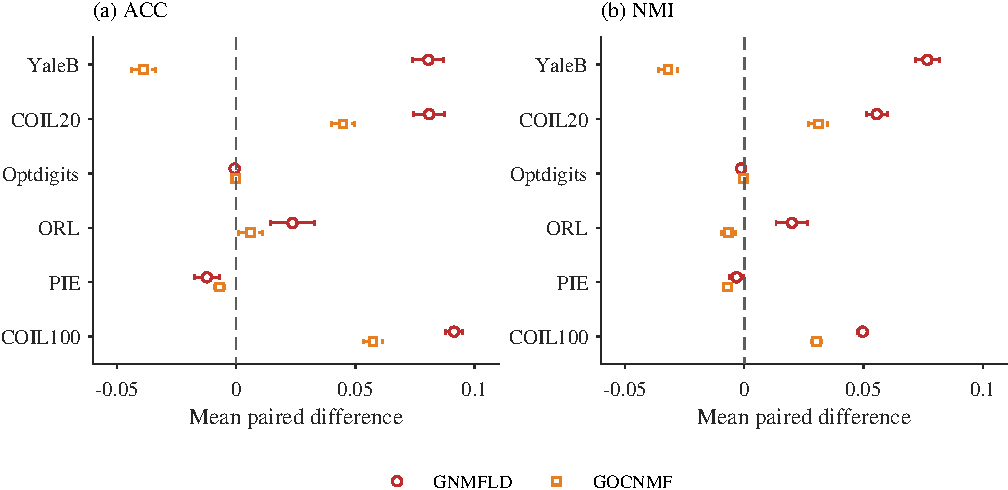
\includegraphics[width=\textwidth]{figures/fig5_paired_differences.pdf}
\caption{Paired performance differences of PCE-NMF relative to GNMFLD and GOCNMF. For baseline $B$ and metric $M$, let
$\Delta_B=M(\mathrm{PCE\mbox{-}NMF})-M(B)$, where
$B\in\{\mathrm{GNMFLD},\mathrm{GOCNMF}\}$ and
$M\in\{\mathrm{ACC},\mathrm{NMI}\}$. Panels (a) and (b) report ACC and NMI,
respectively. Markers and error bars show the mean and the interval
$\overline{\Delta}_B\pm t_{0.975,19}s_{\Delta}/\sqrt{20}$ over the matched
seeds. The dashed line marks $\Delta_B=0$, and
positive values favor PCE-NMF. }
\label{fig:paired_differences}
\end{figure*}

On Optdigits, the differences between PCE-NMF and GOCNMF are below
$5\times10^{-4}$, while HLPNMF has the highest mean ACC and NMI. On ORL,
PCE-NMF attains the highest ACC, whereas HLPNMF attains the highest NMI.

\subsection{Parameter sensitivity}
\label{subsec:sensitivity}

We perform a sensitivity analysis on YaleB, COIL20, and COIL100 using the 10
development seeds. We vary $\lambda\in\{0.01,0.1,1,10,100,1000\}$ at the
locked neighborhood size, and vary $p\in\{2,3,4,5,6\}$ at $\lambda=100$.
All other splits, initializations, updates, and unlabeled-only evaluations are
unchanged. Figure~\ref{fig:parameter_sensitivity} reports native PCE-NMF ACC
and NMI; open circles mark the settings subsequently fixed for the 20-seed
test comparison.

\begin{figure*}[t]
\centering
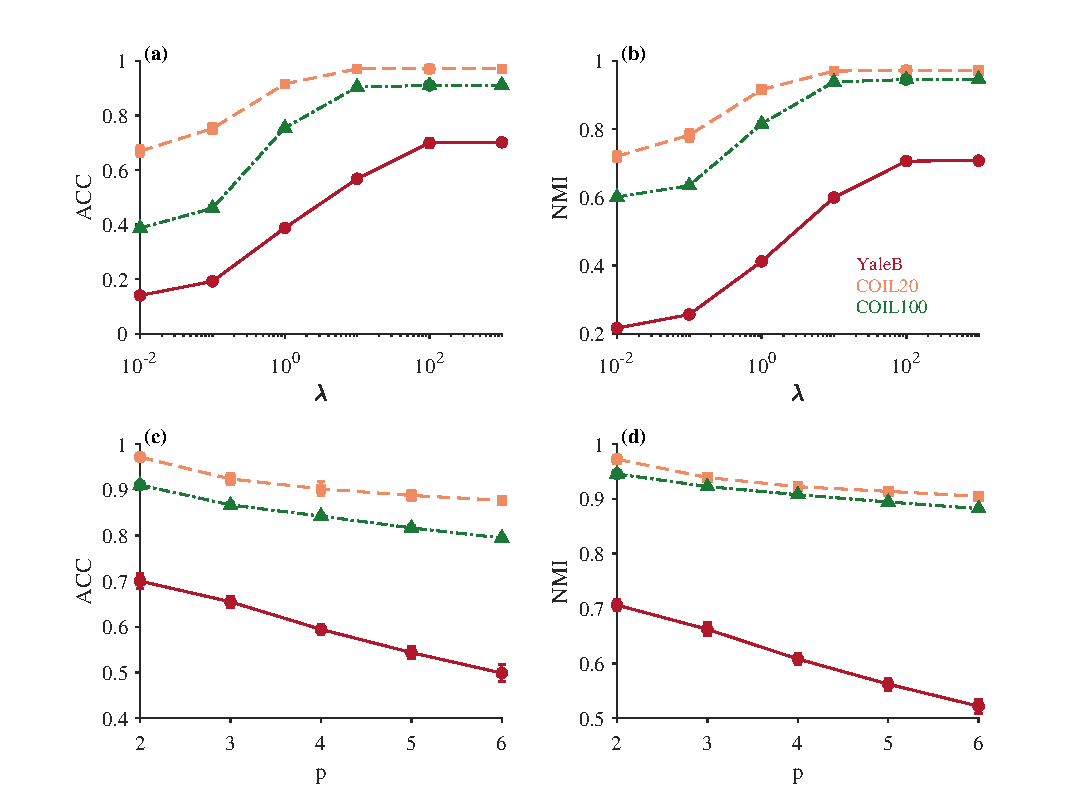
\includegraphics[width=\textwidth,trim=0 13 0 22,clip]{figures/fig7_parameter_sensitivity.pdf}
\caption{Parameter sensitivity of PCE-NMF over 10 paired seeds.
(a,b) ACC and NMI versus $\lambda$ at the locked $p$; (c,d) ACC and NMI
versus $p$ at $\lambda=100$. Error bars show one standard deviation and open
circles mark the settings fixed before the 20-seed test comparison.}
\label{fig:parameter_sensitivity}
\end{figure*}

Performance increases sharply between $\lambda=0.01$ and $10$, and changes
only slightly from $\lambda=100$ to $1000$. At $\lambda=100$, the mean direct
ACC values are $0.7000$, $0.9710$, and $0.9104$ on YaleB, COIL20, and COIL100;
at $\lambda=1000$ they are $0.7017$, $0.9709$, and $0.9114$. The setting
$\lambda=100$ therefore lies on a broad performance plateau.

The neighborhood size is more influential. All three data sets attain their
highest tested mean ACC at $p=2$. Relative to $p=3$, direct ACC increases
from $0.9235$ to $0.9712$ on COIL20 and from $0.8665$ to $0.9103$ on
COIL100. The 20-seed comparison uses $p=2$ for YaleB, COIL20, and COIL100.


\subsection{Influence of supervisory information}

Because PCE-NMF is designed to propagate limited class evidence,
we perform a label-rate robustness analysis under different amounts of
supervision. YaleB, COIL20, and COIL100 provide one face data set and two
object data sets with 20 and 100 classes, respectively, and therefore expose
both data-type and class-count changes within a tractable repeated experiment.
The labeled proportion per class is varied over
$\{5\%,10\%,15\%,20\%\}$ using nested labeled sets, while a common
evaluation pool is retained for all proportions within each paired
trial. Figure~\ref{fig:label_ratio} reports the mean ACC and NMI over
20 paired seeds. SNMFWLP is evaluated by applying 50-start $K$-means to its
learned representation in every trial, consistent with its native prediction
protocol.

\begin{figure*}[!t]
    \centering
    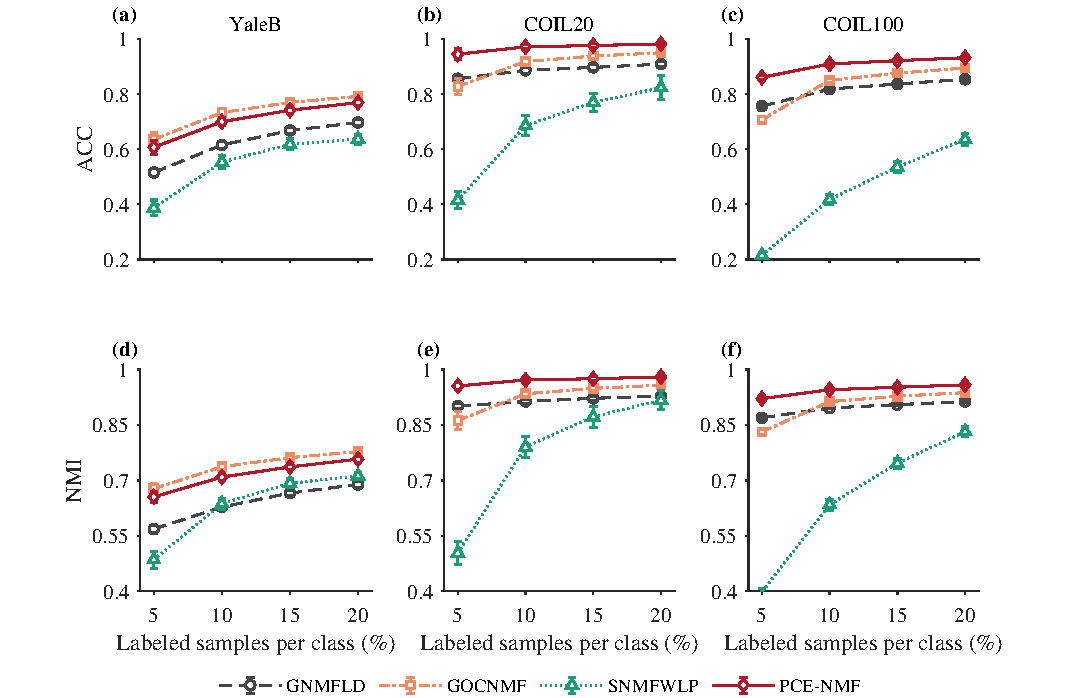
\includegraphics[width=0.9\textwidth]{PCE_label_ratio_ACC_NMI.pdf}
    \caption{Influence of the proportion of labeled samples on clustering
    performance. The upper row reports ACC and the lower row reports NMI
    on YaleB, COIL20, and COIL100. For each paired seed, the labeled sets
    are nested across $5\%$, $10\%$, $15\%$, and $20\%$ supervision,
    while all settings share a common evaluation pool. Markers denote
    the mean results over the separate 20-seed robustness analysis
    (20260617--20260636), and error bars indicate one
    standard deviation. SNMFWLP uses 50-start $K$-means on its learned
    representation.}
    \label{fig:label_ratio}
\end{figure*}

The benefit of propagated class exclusion is most pronounced in the
low-supervision regime. On COIL20 with only $5\%$ labeled samples,
PCE-NMF achieves an ACC of $0.9446$, compared with $0.8274$ for
GOCNMF, while the corresponding NMI values are $0.9555$ and $0.8620$.
The advantage is even more evident on COIL100, where PCE-NMF improves
ACC from $0.7063$ to $0.8602$ and NMI from $0.8312$ to $0.9210$.

PCE-NMF remains ahead of GOCNMF across the four tested supervision levels on
COIL20 and COIL100. Its performance increases with the labeled proportion,
while the largest absolute gains over GOCNMF occur in the low-supervision
regime.

On YaleB, GOCNMF remains stronger over all four supervision levels, and
PCE-NMF consistently outperforms GNMFLD and SNMFWLP.
The strongest PCE-NMF gains in this analysis occur in
low-supervision object-clustering problems with many classes.


\subsection{Ablation of propagated class exclusion}
\label{subsec:hce_ablation}

To isolate the contribution of propagated class exclusion, we compare PCE-NMF
with a hard-class-exclusion variant, denoted HCE-NMF. HCE-NMF preserves the
same factorization structure and the labeled wrong-class zero constraints but
sets the propagated-exclusion regularization weight to zero. This comparison
measures the incremental effect of the complete propagated-exclusion term over
the hard-support model.

Both variants have class-semantic latent coordinates and are evaluated using
the native class-energy decision
\begin{equation}
    \widehat y_i=\arg\max_k \lVert u_k\rVert_2^2v_{ik}^2,
\end{equation}
without permutation alignment. Both variants use the same seeds, labeled
splits, initial factors, cosine graphs, updates, and NMI definition. Table~\ref{tab:hce_ablation} reports the ablation results over the
20 paired trials.

\begin{table}[t]
\centering
\caption{Ablation of propagated class exclusion under the native direct
class-energy decision. Values are mean $\pm$ standard deviation over 20 paired
trials.}
\label{tab:hce_ablation}
\small
\setlength{\tabcolsep}{4.2pt}
\resizebox{\columnwidth}{!}{%
\begin{tabular}{lcccc}
\toprule
& \multicolumn{2}{c}{HCE-NMF} & \multicolumn{2}{c}{PCE-NMF} \\
\cmidrule(lr){2-3}\cmidrule(lr){4-5}
Data set & ACC & NMI & ACC & NMI \\
\midrule
YaleB     & $0.1331\pm0.0119$ & $0.2125\pm0.0129$ & $0.6933\pm0.0157$ & $0.7018\pm0.0114$ \\
COIL20    & $0.6582\pm0.0144$ & $0.7132\pm0.0132$ & $0.9678\pm0.0084$ & $0.9684\pm0.0047$ \\
Optdigits & $0.6538\pm0.0930$ & $0.6090\pm0.0490$ & $0.9833\pm0.0014$ & $0.9579\pm0.0029$ \\
ORL       & $0.2769\pm0.0275$ & $0.5129\pm0.0195$ & $0.6358\pm0.0244$ & $0.7872\pm0.0107$ \\
PIE       & $0.3382\pm0.0191$ & $0.5081\pm0.0170$ & $0.9307\pm0.0130$ & $0.9482\pm0.0066$ \\
COIL100   & $0.3735\pm0.0094$ & $0.5978\pm0.0066$ & $0.9077\pm0.0051$ & $0.9443\pm0.0025$ \\
\bottomrule
\end{tabular}
}
\end{table}

PCE-NMF improves both metrics on every data set. The mean ACC gains over
HCE-NMF range from $0.3097$ on COIL20 to $0.5925$ on PIE, while the NMI gains
range from $0.2552$ to $0.4893$. PCE-NMF wins all 120 seed-level comparisons
for each metric. All 12 data-set--metric tests remain significant after Holm
correction (adjusted $p=2.29\times10^{-5}$). These results show that hard
compatibility constraints alone are insufficient in this model: propagation
supplies useful class-incompatibility information for unlabeled samples.

To separate this gain from the predictive strength of harmonic propagation
itself, we also evaluate a propagation-only control. It uses the same graph,
labeled split, and component-wise harmonic field as PCE-NMF and predicts
\begin{equation}
    \widehat y_i^{\rm LP}=\arg\max_k P_{ik}.
\end{equation}
For a connected component without a labeled anchor, all entries of $P_{i:}$
are zero; such samples are assigned to the most frequent class in the labeled
set, with ties resolved by the smallest class index. The evaluation set is
therefore identical for LP-only and PCE-NMF.

\begin{table}[t]
\centering
\caption{Harmonic propagation alone and PCE-NMF under native class-semantic
decisions. Values are mean $\pm$ standard deviation over the 20 independent
test seeds.}
\label{tab:lp_only}
\small
\setlength{\tabcolsep}{3.8pt}
\resizebox{\columnwidth}{!}{%
\begin{tabular}{lcccc}
\toprule
& \multicolumn{2}{c}{Harmonic LP-only} & \multicolumn{2}{c}{PCE-NMF} \\
\cmidrule(lr){2-3}\cmidrule(lr){4-5}
Data set & ACC & NMI & ACC & NMI \\
\midrule
YaleB     & $0.7365\pm0.0125$ & $0.7384\pm0.0086$ & $0.6933\pm0.0157$ & $0.7018\pm0.0114$ \\
COIL20    & $0.9546\pm0.0099$ & $0.9566\pm0.0068$ & $0.9678\pm0.0084$ & $0.9684\pm0.0047$ \\
Optdigits & $0.9837\pm0.0013$ & $0.9588\pm0.0028$ & $0.9833\pm0.0014$ & $0.9579\pm0.0029$ \\
ORL       & $0.6236\pm0.0245$ & $0.7913\pm0.0091$ & $0.6358\pm0.0244$ & $0.7872\pm0.0107$ \\
PIE       & $0.9488\pm0.0124$ & $0.9628\pm0.0060$ & $0.9307\pm0.0130$ & $0.9482\pm0.0066$ \\
COIL100   & $0.8849\pm0.0079$ & $0.9326\pm0.0039$ & $0.9077\pm0.0051$ & $0.9443\pm0.0025$ \\
\bottomrule
\end{tabular}}
\end{table}

PCE-NMF improves both metrics over LP-only on COIL20 and COIL100, with mean
gains of $0.0133/0.0118$ and $0.0228/0.0117$ in ACC/NMI, respectively. It
also improves ACC on ORL by $0.0122$, while LP-only has $0.0040$ higher NMI.
LP-only is stronger on YaleB and PIE. On Optdigits, the absolute differences
are $4.0\times10^{-4}$ ACC and $9.2\times10^{-4}$ NMI. All 12 paired tests
remain significant after Holm correction; the adjusted values are
$7.84\times10^{-4}$ for both Optdigits metrics and at most this value for the
other comparisons. Harmonic evidence is already a strong classifier, while
its coupling to contribution-energy shrinkage supplies the additional gains
on COIL20 and COIL100.

Figure~\ref{fig:pce_mechanism} traces this mechanism in a formal COIL20 trial.
The harmonic evidence concentrates near the correct class coordinate, its
complement assigns small exclusion weight to that coordinate and large weights
to incompatible coordinates, and the learned class-energy share becomes
strongly diagonal. Thus the observed gain is accompanied by the matrix pattern
predicted by the PCE penalty.

\begin{figure*}[t]
\centering
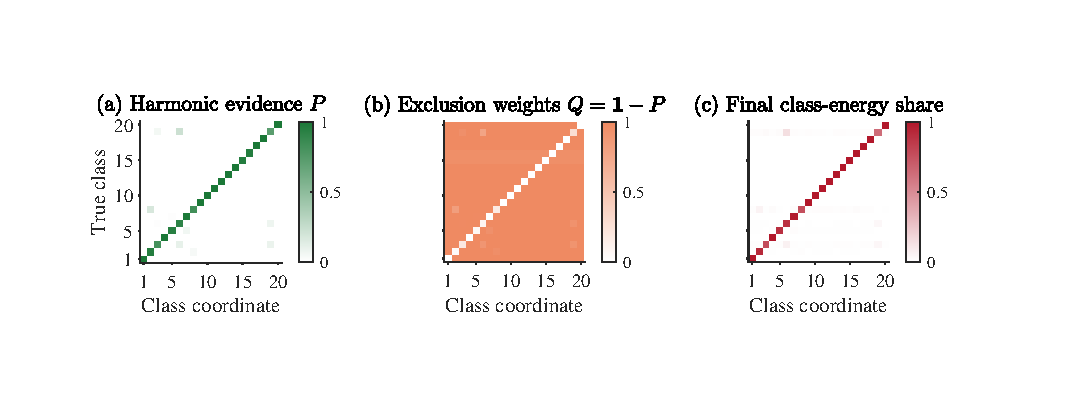
\includegraphics[width=0.9\textwidth,trim=0 41 0 45,clip]{figures/fig2_pce_mechanism_heatmaps.pdf}
\caption{Propagation-to-factorization mechanism on COIL20 for development seed 20260617,
$p=2$, $\lambda=100$, and 50 iterations. Each row averages all unlabeled
samples of one true class. (a) Harmonic class evidence $P$; (b) propagated
exclusion weights $Q=1-P$; and (c) the final normalized class-energy share
$s_{ik}/\sum_j s_{ij}$.}
\label{fig:pce_mechanism}
\end{figure*}

\subsection{Sample-level visualization of propagated exclusion}
\label{sec:sample_mechanism_visualization}

Figure~\ref{fig:sample_mechanism} presents three sample-level mechanism cases
from the propagation-to-decision path on ORL. The samples are selected deterministically by
scanning the true classes and sample indices and retaining the first sample
from each of the first three classes for which HCE-NMF is incorrect and
PCE-NMF is correct. All quantities come from the same labeled split,
initialization, graph, and seed used by the paired ablation. The harmonic
evidence $P_{i:}$ identifies compatible class coordinates, and
$Q_{i:}=\mathbf{1}-P_{i:}$ assigns larger exclusion weights to incompatible
coordinates. The final two columns show the normalized class-contribution
energies
\begin{equation}
    \bar{s}_{ik}=\frac{\lVert u_k\rVert_2^2v_{ik}^2}
    {\sum_j\lVert u_j\rVert_2^2v_{ij}^2}.
\end{equation}

\begin{figure*}[!t]
\centering
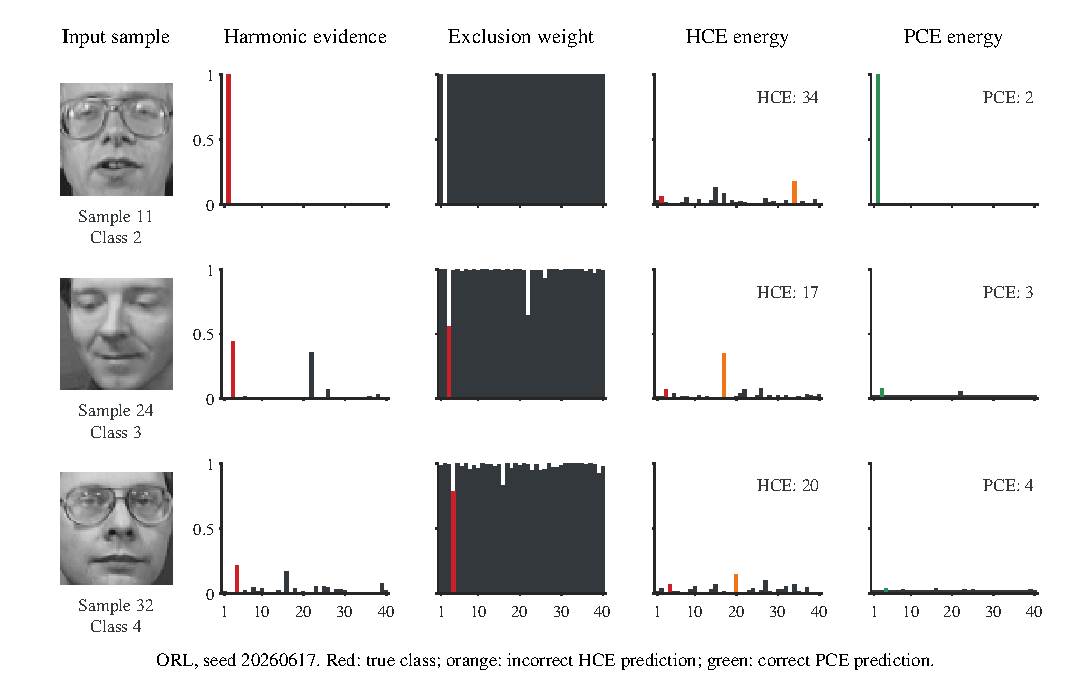
\includegraphics[width=0.91\textwidth]{figures/fig6_sample_mechanism_preview_orl.pdf}
\caption{Three sample-level cases of the
propagated-exclusion mechanism on ORL for development seed
20260617, $p=3$, $\lambda=100$, and 50 iterations. The rows show samples 11,
24, and 32, whose true classes are 2, 3, and 4. From left to right: input
sample, harmonic class evidence, propagated exclusion weight, normalized
HCE-NMF class energy, and normalized PCE-NMF class energy. Red marks the true
class coordinate, orange marks the incorrect HCE-NMF decision, and green marks
the correct PCE-NMF decision. HCE-NMF predicts classes 34, 17, and 20, whereas
PCE-NMF predicts classes 2, 3, and 4.}
\label{fig:sample_mechanism}
\end{figure*}

For these cases, HCE-NMF distributes substantial energy over
several incompatible coordinates and assigns the largest energy to an
incorrect class. Propagated exclusion suppresses these competing coordinates
and moves the largest normalized contribution energy to the true class. This
sample-level transition illustrates the mechanism, while the paired ablation
in Table~\ref{tab:hce_ablation} provides the corresponding performance evidence
over all seeds.

\subsection{Visualization of learned representations}
\label{subsec:embedding_visualization}

We visualize the scale-invariant representations learned on COIL100, where
PCE-NMF ranks first in both ACC and NMI in the formal comparison. For
sample $i$, the representation is
\begin{equation}
    z_{ik}=\lVert u_k\rVert_2v_{ik},\qquad k=1,\ldots,c,
\end{equation}
so that $z_{ik}^2$ equals the class-wise contribution energy used by the
PCE-NMF decision rule. This representation is unchanged by the standard NMF
diagonal scaling transformation.

\begin{figure*}[!t]
\centering
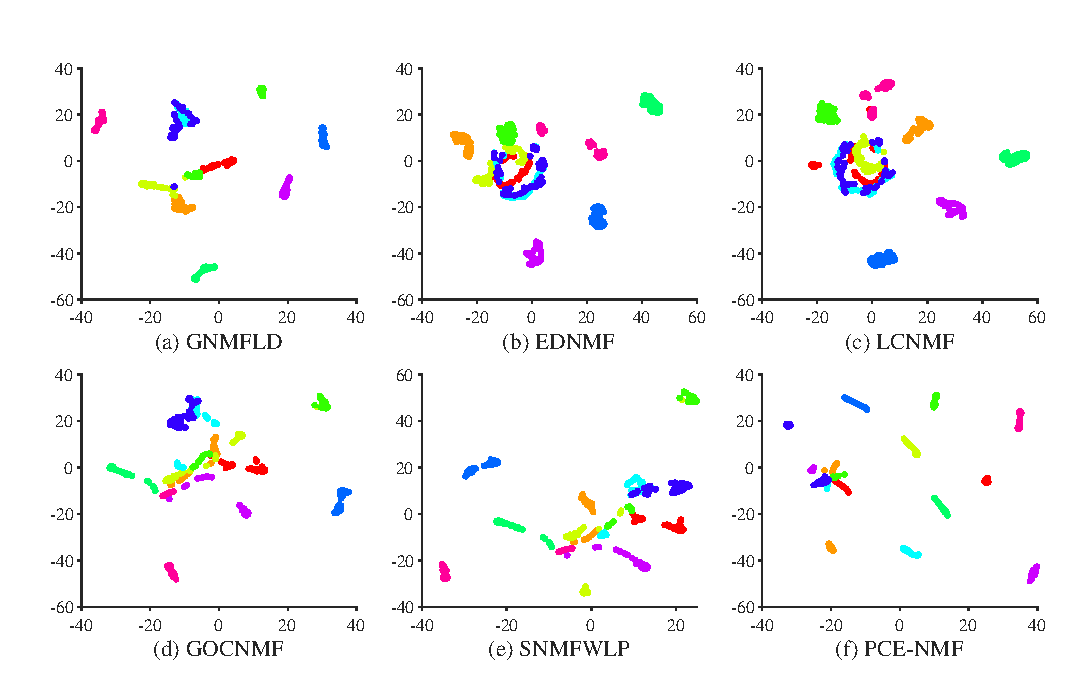
\includegraphics[width=0.90\textwidth]{figures/fig7_scale_invariant_embeddings.pdf}
\caption{Two-dimensional visualization of scale-invariant representations for
ten prespecified COIL100 classes: (a) GNMFLD, (b) EDNMF, (c) LCNMF,
(d) GOCNMF, (e) SNMFWLP, and (f) PCE-NMF. The plots use the same unlabeled
samples, class colors, t-SNE configuration, and development seed 20260617. Each
representation is mapped independently using Euclidean distance, perplexity
30, and no input standardization. Each independently fitted panel has its own
coordinate system and provides a qualitative within-panel view.}
\label{fig:embeddings}
\end{figure*}

Figure~\ref{fig:embeddings} shows the local structure within each learned
representation. Each t-SNE panel has an independent orientation, scale, and
coordinate system. Table~\ref{tab:pce_external_baselines} reports ACC and NMI
computed from the original representations.

\subsection{Empirical convergence behavior}
\label{subsec:convergence}

We record the PCE-NMF objective for 50 iterations on YaleB, COIL20, and
COIL100 using the 10 development seeds and the formal parameters.
Figure~\ref{fig:convergence} shows the mean normalized objective
$F^{(t)}/F^{(1)}$.

\begin{figure*}[!t]
\centering
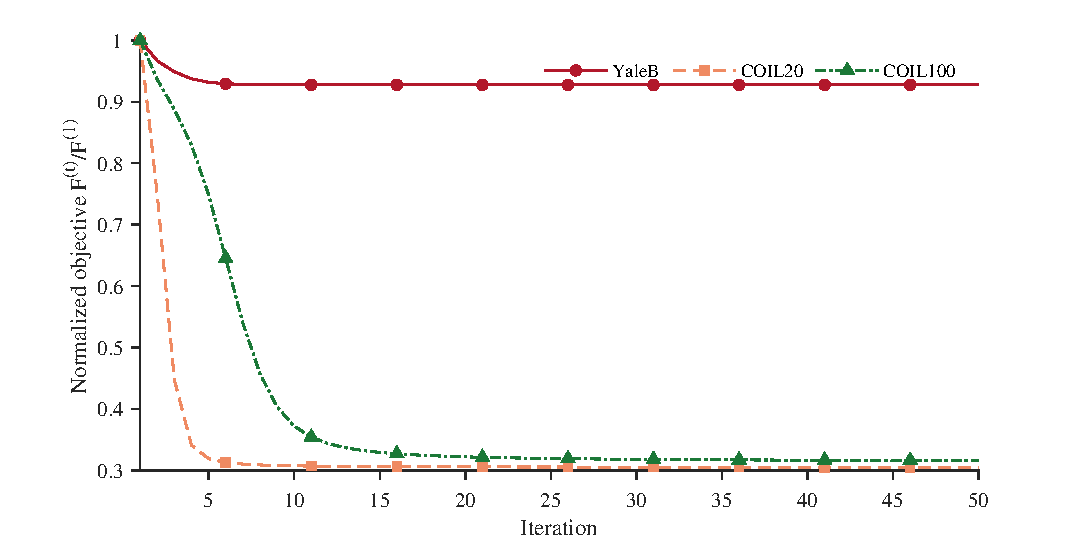
\includegraphics[width=0.62\textwidth,trim=0 2 0 15,clip]{figures/fig8_convergence_curves.pdf}
\caption{Mean objective trajectories of PCE-NMF over the 10 development seeds at the
formal settings. Curves show $F^{(t)}/F^{(1)}$; sparse markers distinguish the
three data sets.}
\label{fig:convergence}
\end{figure*}

All 30 recorded trajectories are finite and nonincreasing under the numerical
tolerance used by the implementation. At iteration 50, the mean ratios
$F^{(50)}/F^{(1)}$ are $0.9276$, $0.3051$, and $0.3160$ on YaleB, COIL20, and
COIL100, respectively. The corresponding mean relative changes in the final
step are $1.60\times10^{-7}$, $2.61\times10^{-5}$, and
$1.74\times10^{-4}$. These measurements establish objective-value descent for
the recorded runs.







\subsection{Propagation coverage and constraint diagnostics}
\label{subsec:diagnostics}

The harmonic field is defined component-wise, and propagated
class-exclusion weights are introduced only on connected components
that contain at least one labeled anchor. An unanchored component contains no
label information for class-evidence inference, so PCE-NMF assigns zero
propagated-exclusion weight to that component.

Across the 20 independent test seeds, the mean anchor coverage is $1.000$ on
YaleB, $0.985$ on COIL20, $1.000$ on Optdigits, $0.940$ on ORL, $0.994$ on
PIE, and $0.962$ on COIL100. The corresponding minimum coverage values are
$1.000$, $0.975$, $1.000$, $0.919$, $0.979$, and $0.944$,
respectively. Thus, all unlabeled samples are anchored on YaleB and Optdigits,
while only a small fraction of samples belongs to unanchored components on
the other four data sets. The minimum observed coverage remains above $0.91$
on every data set.
These results show that the harmonic evidence reaches the great
majority of unlabeled samples under the graph settings used in the
formal experiments, while the component-wise construction prevents
unsupported class evidence from being assigned to disconnected
regions.

We further examine numerical feasibility of the constrained
factorization. All 1080 method runs return finite factors and finite
evaluation metrics. For PCE-NMF, the labeled wrong-class entries are reset
to zero after every multiplicative update, and the recorded support-violation
field is zero in all runs. The same holds for LCNMF, which also imposes hard
wrong-class support constraints. Hence, the implemented updates preserve the
prescribed support structure.
Together, the coverage and feasibility diagnostics confirm that the
propagated evidence is applied only where labeled information is
available and that the hard exclusion constraints are maintained
consistently during optimization.

\subsection{Discussion}
\label{subsec:experiment_discussion}

The experiments separate two sources of supervision. Hard support constraints
assign class semantics to labeled coordinates, while propagated exclusion
extends class-incompatibility information to unlabeled samples. Removing the
second source produces large losses on every data set and every paired seed.
The diagonal patterns in Fig.~\ref{fig:pce_mechanism} connect this performance
change to the intended sequence from harmonic evidence to exclusion weights
and class-energy concentration.

The external comparison shows complementary strengths among PCE-NMF, GOCNMF,
and HLPNMF. HLPNMF leads on YaleB, Optdigits, and PIE; PCE-NMF leads on both
metrics for COIL20 and COIL100 and on ACC for ORL; HLPNMF leads on ORL NMI.
The comparison therefore separates regimes favored by harmonic exclusion,
one-hot graph smoothing, and high-order hypergraph propagation. The
label-rate analysis shows the largest PCE-NMF gains on the
multi-class object data at the lowest examined label rate, with smaller gaps
as direct supervision increases.

The external ranking uses the same permutation-aligned ACC definition for all
methods. The native PCE-NMF decision in Eq.~\eqref{eq:prediction} gives the
same mean ACC on YaleB, COIL20, Optdigits, and PIE; the mean absolute gap is
$1.59\times10^{-3}$ on COIL100 and $0.0110$ on ORL. Hence the class-semantic coordinates support direct prediction while the
aligned score preserves a common clustering comparison.

The LP-only control clarifies what is supplied by the harmonic field and what
is supplied by its coupling with NMF. Harmonic propagation alone is strongest
on YaleB and PIE and is effectively tied with PCE-NMF on Optdigits. PCE-NMF
adds clear gains on COIL20 and COIL100 and improves ORL ACC. The factorization
therefore contributes most on the two multi-class object data sets, whereas
the propagated evidence itself accounts for much of the performance on the
face and digit data. The proposed penalty therefore contributes a distinct
factorization gain on the two multi-class object data sets.

Graph construction controls how far class evidence travels. The $\lambda$
curves place $\lambda=100$ on a broad plateau, whereas the neighborhood curves
show large changes from $p=3$ to $p=2$ on COIL20 and COIL100. Thus, $p$ is the
principal graph parameter. The neighborhood values in Table~\ref{tab:datasets}
are used consistently in the main comparison, ablation, and label-rate
robustness analysis.

The objective trajectories, anchor-coverage measurements, and zero-support
diagnostics connect the mathematical model to the executed algorithm. They
show monotonic finite-precision descent in all recorded trajectories, broad
reach of the harmonic evidence, and exact preservation of labeled wrong-class
zeros.

The data-set pattern distinguishes the regimes favored by the strongest
mechanisms. HLPNMF leads on the YaleB and PIE face data and on Optdigits,
whereas PCE-NMF shows its largest gains on COIL20 and COIL100 under low
supervision. Across
the three label-rate data sets, this advantage decreases as direct supervision
increases. Neighborhood size has a larger effect than $\lambda$ on COIL20 and
COIL100, establishing graph calibration as the principal model-selection
step. The blocked neighbor search and sparse harmonic solve provide the
computational route for extending PCE-NMF beyond the largest collection tested
here ($n=7200$).




\section{Conclusion}
\label{sec:conclusion}

PCE-NMF converts harmonic class evidence into a class-incompatibility field
and applies it to diagonal-scale-invariant rank-one contribution energies.
The same energies define a direct class decision, linking supervision,
factorization, and assignment through one mathematical quantity. The
canonical representation expresses this mechanism as sample- and
class-specific quadratic shrinkage, and the ideal alternating updates
generate a non-increasing objective sequence on the stated positive domain.
Across six data sets and nine tested methods, PCE-NMF achieves the highest
mean ACC and NMI on COIL20 and COIL100 and the highest ACC on ORL. HLPNMF
leads on YaleB, Optdigits, and PIE, and on ORL NMI. The HCE-NMF ablation establishes the value of propagated
exclusion beyond hard class support. The LP-only comparison further shows
where factorization adds value: PCE-NMF improves both metrics on COIL20 and
COIL100, while harmonic propagation alone is stronger on YaleB and PIE and
is nearly equal on Optdigits. The main empirical benefit is therefore
concentrated in low-supervision multi-class object clustering. Propagated
class exclusion provides a direct route from partial labels to class-semantic
NMF clustering and a scale-invariant mechanism for coupling propagation with
non-negative factorization.



\section*{CRediT authorship contribution statement}

\noindent Deshu Sun: Writing--original draft, Methodology, Software,
Conceptualization, Formal analysis.\\
Feng Wang: Writing--review and editing, Funding acquisition, Visualization,
Conceptualization. All authors reviewed the manuscript.


\section*{Declaration of competing interest}
The authors declare that they have no known competing financial interests or personal relationships that could have appeared to influence the work reported in this paper.

\section*{Data and code availability}

The PCE-NMF solver, formal protocol, independent-test trial records, analysis
scripts, and figure source data are available at
\url{https://github.com/matrix-research-lab-Wf/PCE-NMF}. The six benchmark
data sets are available from the original providers cited in
Section~\ref{subsec:data_protocol}; their redistribution terms are retained.
The repository distributes the PCE-NMF implementation. Third-party baseline
implementations are obtained from their respective authors or official
repositories.

\section*{Acknowledgments}
This work was supported by Guizhou Provincial Science and Technology Projects (2025039, 2026283), the High-Level Innovative Talent Project of Guizhou Province (GCC2023027), the Natural Science Research Project of Department of Education of Guizhou Province (2024259), and the Research Foundation of Guizhou Minzu University (GZMUZK[2023]YB10).


%%%%%%%%%%%%%%%%%%%%%%%%%%%%%%%%%%%%%%%%%%%%%%%%%%%%%%%%%%%%%%%%%%%

\balance
\footnotesize
\begin{thebibliography}{99}

\bibitem{Lee1999NMF}
Lee, D.~D., Seung, H.~S., 1999.
Learning the parts of objects by non-negative matrix factorization.
\emph{Nature} 401(6755), 788-791.

\bibitem{Lee2001Algorithms}
Lee, D.~D., Seung, H.~S., 2000.
Algorithms for non-negative matrix factorization.
In: \emph{Advances in Neural Information Processing Systems 13}, pp.~556-562.

\bibitem{Liu2012CNMF}
Liu, H., Wu, Z., Li, X., Cai, D., Huang, T.~S., 2012.
Constrained nonnegative matrix factorization for image representation.
\emph{IEEE Transactions on Pattern Analysis and Machine Intelligence} 34~(7), 1299-1311.

\bibitem{Xing2021DSSNMF}
Xing, Z., Wen, M., Peng, J., Feng, J., 2021.
Discriminative semi-supervised non-negative matrix factorization for data clustering.
\emph{Engineering Applications of Artificial Intelligence} 103, 104289.

\bibitem{Li2025EDNMF}
Li, J., Shen, X., Li, C., Li, Y., 2025.
Elements discriminative non-negative matrix factorization for data clustering.
\emph{Engineering Applications of Artificial Intelligence} 156, 111210.

\bibitem{Li2025GOCNMF}
Li, J., Li, C., 2025.
Graph regularized one-hot-constrained nonnegative matrix factorization for data representation.
\emph{Engineering Applications of Artificial Intelligence} 156, 111224.

\bibitem{Shen2026LCNMF}
Shen, X., Li, J., 2026.
Locally constrained non-negative matrix factorization for data clustering.
\emph{IEEE Access} 14, 78907-78919.

\bibitem{Wang2015ConstraintNMF}
Wang, D., Gao, X., Wang, X., 2016.
Semi-supervised nonnegative matrix factorization via constraint propagation.
\emph{IEEE Transactions on Cybernetics} 46~(1), 233-244.

\bibitem{Yin2023HSSNMF}
Yin, J., Peng, S., Yang, Z., Chen, B., Lin, Z., 2023.
Hypergraph based semi-supervised symmetric nonnegative matrix factorization for image clustering.
\emph{Pattern Recognition} 137, 109274.

\bibitem{Yang2025SPNMF}
Yang, X., Zhu, T., Peng, S., Nie, F., Lin, Z., 2025.
Semi-supervised pivotal-aware nonnegative matrix factorization with label and pairwise constraint propagation for data clustering.
\emph{Pattern Recognition} 157, 110933.

\bibitem{Mo2024PNLPSCNMF}
Mo, Y., Li, X., Mei, J., 2024.
Semi-supervised nonnegative matrix factorization with label propagation and constraint propagation.
\emph{Engineering Applications of Artificial Intelligence} 133, 108196.

\bibitem{Jing2026SNMFWLP}
Jing, W., Lu, L., Ou, W., 2026.
Semi-supervised non-negative matrix factorization with weighted label propagation for data representation.
\emph{Signal Processing} 241, 110407.

\bibitem{Li2026HLPNMF}
Li, J., Zhou, X., Shen, X., Li, C., 2026.
High-order label propagation-guided nonnegative matrix factorization for semi-supervised clustering.
\emph{Pattern Recognition} 180, 114657.

\bibitem{Peng2021CSNMF}
Peng, S., Ser, W., Chen, B., Lin, Z., 2021.
Robust semi-supervised nonnegative matrix factorization for image clustering.
\emph{Pattern Recognition} 111, 107683.

\bibitem{Zhu2003Harmonic}
Zhu, X., Ghahramani, Z., Lafferty, J., 2003.
Semi-supervised learning using Gaussian fields and harmonic functions.
In: \emph{Proceedings of the 20th International Conference on Machine Learning}, pp.~912-919.

\bibitem{Georghiades2001YaleB}
Georghiades, A.~S., Belhumeur, P.~N., Kriegman, D.~J., 2001.
From few to many: illumination cone models for face recognition under variable lighting and pose.
\emph{IEEE Transactions on Pattern Analysis and Machine Intelligence} 23~(6), 643--660.

\bibitem{Nene1996COIL20}
Nene, S.~A., Nayar, S.~K., Murase, H., 1996.
Columbia Object Image Library (COIL-20).
Technical Report CUCS-005-96, Columbia University.

\bibitem{Alpaydin1998Optdigits}
Alpaydin, E., Kaynak, C., 1998.
Optical Recognition of Handwritten Digits [Dataset].
UCI Machine Learning Repository. \url{https://doi.org/10.24432/C50P49}.

\bibitem{Samaria1994ORL}
Samaria, F.~S., Harter, A.~C., 1994.
Parameterisation of a stochastic model for human face identification.
In: \emph{Proceedings of the 2nd IEEE Workshop on Applications of Computer Vision}, pp.~138--142.

\bibitem{Sim2003PIE}
Sim, T., Baker, S., Bsat, M., 2003.
The CMU Pose, Illumination, and Expression database.
\emph{IEEE Transactions on Pattern Analysis and Machine Intelligence} 25~(12), 1615--1618.

\bibitem{Nene1996COIL100}
Nene, S.~A., Nayar, S.~K., Murase, H., 1996.
Columbia Object Image Library (COIL-100).
Technical Report CUCS-006-96, Columbia University.

\bibitem{Xing2021GNMFLD}
Xing, Z., Ma, Y., Yang, X., Nie, F., 2021.
Graph regularized nonnegative matrix factorization with label discrimination for data clustering.
\emph{Neurocomputing} 440, 297-309.

\bibitem{Wilcoxon1945}
Wilcoxon, F., 1945.
Individual comparisons by ranking methods.
\emph{Biometrics Bulletin} 1~(6), 80-83.

\end{thebibliography}


\end{document}
